%%
% The BIThesis Template for Bachelor Paper Translation
%
% 北京理工大学毕业设计(论文) —— 使用 XeLaTeX 编译
%
% Copyright 2020-2023 BITNP
%
% This work may be distributed and/or modified under the
% conditions of the LaTeX Project Public License, either version 1.3
% of this license or (at your option) any later version.
% The latest version of this license is in
%   http://www.latex-project.org/lppl.txt
% and version 1.3 or later is part of all distributions of LaTeX
% version 2005/12/01 or later.
%
% This work has the LPPL maintenance status `maintained'.
%
% The Current Maintainer of this work is Feng Kaiyu.
%
% Compile with: xelatex -> biber -> xelatex -> xelatex
%%

% !TeX program = xelatex
% !BIB program = biber


\documentclass[type=bachelor_translation]{bithesis}

\BITSetup{
  cover = {
    % 在封面中载入有「北京理工大学」字样的图片,如无必要请勿改动。
    headerImage = images/header.png,
    % 在封面标题中使用思源黑体,使用此选项可以保证与 Word 封面标题的字体一致。
    xiheiFont = STXIHEI.TTF,
    % 官方模板采用了固定的下划线宽度。我们采用以下两个选项来达成这个效果。
    % 如果你想要使用自动计算的下划线宽度,也可以删去以下两个选项。
    autoWidth = false,
    valueMaxWidth = 20em,
  },
  info = {
    title = 基于深度学习和聚类优化的多实例点云配准,
    titleEn = {Optimized Multi-Instance Point Cloud Registration based on
    Deep Learning and Cluster Methods
    },
    % 想要删除某项封面信息,直接删除该项即可。
    % 想要让某项封面信息留空(但是保留下划线),请设置为空字符串。
    % 如需要换行,则用 “\\” 符号分割。
    school = 自动化学院,
    major = 自动化,
    author = 杨润一,
    class = 06011902,
    studentId = 1120191211,
    supervisor = 由育阳,
    translationTitle = Geometrc Transformer: 快速且稳健的点云配准,
    translationOriginTitle = Geometric Transformer for Fast and \\ Robust Point Cloud Registration,
    keywords = {点云配准; 描述子; 特征描述; 深度学习; 毕业设计(外文翻译)},
    % 如果你的毕设为校外毕设,请将下面这一行语句解除注释(删除第一个百分号字符)并填写你的校外毕设导师名字
  },
  style = {
    % 保持参考文献的缩进样式与 Word 模板一致。
    % 如果你不需要此样式,请将此行注释掉。
    bibliographyIndent = false,
    % head = {自定义页眉文字}
  }
}

% 有关参考文献的样式可以在此处修改;如无必要无需修改。
\usepackage[
  backend=biber,
  style=gb7714-2015,
  gbalign=gb7714-2015,
  gbnamefmt=lowercase,
  gbpub=false,
  doi=false,
  url=false,
  eprint=false,
  isbn=false,
]{biblatex}

\usepackage{graphicx}
\usepackage{amsmath}
\usepackage{amssymb}
\usepackage{booktabs}

\usepackage{multirow}
\usepackage{xcolor}
\usepackage{array}
\usepackage{multirow}
\usepackage{mathtools}
\usepackage{overpic}
\usepackage{stmaryrd}

% 参考文献引用文件位于 misc/ref.bib
\addbibresource{misc/ref.bib}

% 文档开始
\newcommand\BackgroundPicture{%
  \put(0,0){%
    \parbox[b][\paperheight]{\paperwidth}{%
      \vfill
      \centering%
      
\includegraphics[width=\paperwidth]{images/background.pdf}
      \vfill
    }}}

% 文档开始
\begin{document}
\AddToShipoutPicture{\BackgroundPicture}


% 标题页面:如无特殊需要,本部分无需改动
% \input{misc/0_cover.tex}
\MakeCover

% 前置页面定义
\frontmatter
%%%
% The BIThesis Template for Bachelor Graduation Thesis
%
% 北京理工大学毕业设计(论文)原创性声明模板 —— 使用 XeLaTeX 编译
%
% Copyright 2020-2023 BITNP
%
% This work may be distributed and/or modified under the
% conditions of the LaTeX Project Public License, either version 1.3
% of this license or (at your option) any later version.
% The latest version of this license is in
%   http://www.latex-project.org/lppl.txt
% and version 1.3 or later is part of all distributions of LaTeX
% version 2005/12/01 or later.
%
% This work has the LPPL maintenance status `maintained'.
%
% The Current Maintainer of this work is Feng Kaiyu.
%
% Compile with: xelatex -> biber -> xelatex -> xelatex
%
% 如无特殊需要,本页面无需更改

\MakeOriginality

% 摘要:在摘要相应的 TeX 文件处进行摘要部分的撰写
%%
% The BIThesis Template for Bachelor Graduation Thesis
%
% 北京理工大学毕业设计(论文)中英文摘要 —— 使用 XeLaTeX 编译
%
% Copyright 2020-2023 BITNP
%
% This work may be distributed and/or modified under the
% conditions of the LaTeX Project Public License, either version 1.3
% of this license or (at your option) any later version.
% The latest version of this license is in
%   http://www.latex-project.org/lppl.txt
% and version 1.3 or later is part of all distributions of LaTeX
% version 2005/12/01 or later.
%
% This work has the LPPL maintenance status `maintained'.
%  
% The Current Maintainer of this work is Feng Kaiyu.

% 中英文摘要章节
\begin{abstract}
    三维点云配准是点云处理中的一项基本任务,其在机械臂、自动驾驶、自主运动机器人、即时定位与地图构建(Simultaneous Localization and Mapping,SLAM)等众多基于视觉方法的应用中起着关键的作用。随着人工智能、元宇宙、自动驾驶等技术的兴起,将深度学习应用于点云配准的工作已经日趋成熟。目前大多数点云配准任务研究主要集中在成对配准上。然而,在实际应用中,目标场景可能包含多个重复实例,我们需要估计模板点云与目标点云中这些重复实例之间的多个刚性变换,也就是多实例点云配准。

    本文针对三维点云配准问题,特别是多实例点云配准,进行了深入研究。我们调研并整理了多实例点云配准的国内外研究现状,并总结了前人研究的优势和劣势。现有解决方案需要对大量假设进行采样以检测可能的实例并排除异常值,当实例和异常值的数量增加时,其鲁棒性和效率会显着降低。我们建议根据距离不变矩阵将噪声对应集直接分组到不同的簇中。通过聚类自动识别实例和异常值,达到稳健且快速表现。
    
    基于这一研究背景,我们提出了新的多实例点云配准架构,高效对应聚类的多实例点云配准 (ECC) 。分析聚类方法的点云配准,发现对于描述子的依赖性高,离群点比例高的时候效果会大大下降,所以我们提出了基于深度学习和聚类优化的多实例点云配准 (DMR),首先利用对比学习来学习输入推定对应关系的分布良好的深度表示。然后基于这些表示,我们提出了异常值修剪策略和聚类策略,以有效地删除异常值并将剩余的对应关系分配给正确的实例,达到了更好的效果。
    
    综上所述,我们的研究表明,基于深度学习的多实例点云配准方法在处理复杂的多实例点云配准问题上具有优秀的性能,提供了新的研究思路和方法。
    
\end{abstract}

% 英文摘要章节
\begin{abstractEn}
    Three-dimensional point cloud registration is a fundamental task in point cloud processing, which plays a crucial role in a wide range of vision-based applications such as robotic arms, autonomous driving, autonomous mobile robots, and Simultaneous Localization and Mapping (SLAM). With the rise of artificial intelligence, metaverse, autonomous driving, and other technologies, the application of deep learning to point cloud registration has become increasingly mature. Current research on point cloud registration mostly focuses on pairwise registration. However, in practical applications, the target scene may contain multiple repeated instances, and we need to estimate multiple rigid transformations between the template point cloud and these repeated instances in the target point cloud, that is, multi-instance point cloud registration.

    This paper conducts in-depth research on the problem of three-dimensional point cloud registration, especially multi-instance point cloud registration. We have surveyed and summarized the domestic and international research status of multi-instance point cloud registration and summarized the advantages and disadvantages of previous studies. Existing solutions require sampling a large number of hypotheses to detect possible instances and reject outliers, and their robustness and efficiency degrade significantly when the number of instances and outliers increases. We propose to directly group the noisy correspondence set into different clusters based on a distance invariance matrix. Through clustering, instances and outliers are automatically identified, achieving robust and fast performance.
    
    Based on this research background, we propose a new multi-instance point cloud registration framework, \textbf{E}fficient \textbf{C}orrespondence \textbf{C}lustering for Multi-instance Point Cloud Registration (\textbf{ECC}). After analyzing the point cloud registration of the clustering method, we find that the effect will drop significantly when it has high dependency on the descriptor and a high proportion of outliers. Therefore, we propose \textbf{D}eep Learning and Cluster Opimisation based \textbf{M}ulti-instance Point Cloud \textbf{R}egistration (\textbf{DMR}), which first uses contrastive learning to learn a good deep representation of the input estimation correspondence. Then, based on these representations, we propose an outlier pruning strategy and a clustering strategy to effectively remove outliers and allocate the remaining correspondences to the correct instances, achieving better results.
    
    In conclusion, our research shows that the deep learning-based multi-instance point cloud registration method has excellent performance in dealing with complex multi-instance point cloud registration problems and provides new research ideas and methods.
\end{abstractEn}

% 目录
\MakeTOC

% 正文开始
\mainmatter

% 第一章
%%
% The BIThesis Template for Bachelor Graduation Thesis
%
% 北京理工大学毕业设计(论文)第一章节 —— 使用 XeLaTeX 编译
%
% Copyright 2020-2023 BITNP
%
% This work may be distributed and/or modified under the
% conditions of the LaTeX Project Public License, either version 1.3
% of this license or (at your option) any later version.
% The latest version of this license is in
%   http://www.latex-project.org/lppl.txt
% and version 1.3 or later is part of all distributions of LaTeX
% version 2005/12/01 or later.
%
% This work has the LPPL maintenance status `maintained'.
%
% The Current Maintainer of this work is Feng Kaiyu.
%
% 第一章节

\chapter{绪论}

\section{研究背景和意义}
% 这里插入一个参考文献,仅作参考

\subsection{三维点云配准}
21世纪以来,人工智能技术的发展对于社会有着重大的影响,智能化成为工程技术突破的内核。机器能够进行快速计算、存储和处理大量数据,并通过互联网将社会连为一体。现在由人工智能驱动的新一代机器,它们可以越来越自主地解决复杂的任务,其中以视觉为核心的机器技术快速发展,机械臂、自动驾驶、自主运动机器人等进入了人们的视野。随着2012年AlexNet\cite{krizhevsky2017imagenet} 问世以来,深度学习方法打开了计算机视觉的新大门。越来越多的深度学习方法比如VGG\cite{simonyan2014very} 、ResNet\cite{he2016deep} 、ViT\cite{dosovitskiy2020image} 被用在了图像分类、分割、场景理解等任务中。为了更好的理解真实世界,人们开始尝试将深度学习方法用于三维数据中,随着激光雷达和Kinect等高精度传感器的快速发展,点云已经成为表示三维世界的主要数据格式。2017年PointNet\cite{qi2017pointnet} 出现后,深度学习方法也同样被广泛应用在了点云处理中。

三维点云配准是点云处理中的一项基本任务\cite{qi2017pointnet,huang2021comprehensive,besl1992method} ,其在机械臂、自动驾驶、自主运动机器人等众多基于视觉方法的应用中起着关键的作用。首先是三维重建,生成完整的三维场景是各种计算机视觉应用的基础和重要技术,包括自动驾驶中的高精度三维地图重建、机器人技术中的三维环境重建等。例如,配准可以为机器人应用程序中的路线规划和决策构建三维环境。

其次,三维场景中的定位。三维场景中的定位和重定位对于机器人技术尤其重要。例如,无人驾驶汽车会估计其在地图上的位置及其与道路边界线的距离。点云配准可以将当前的实时三维视图与其所属的三维环境准确匹配,提供高精度定位服务。此应用表明,点云配准提供了机器和三维环境交互一种解决方案。

第三,位姿估计。将点云A与另一个点云B对齐可以生成与点云B相关的点云A的位姿信息。这个位姿信息可用于机器人决策。例如,点云配准可以获取环境中物体的位姿信息,以决定机械臂移动到哪里以准确抓取并移动物体。位姿估计为机器人三维环境理解提供了重要信息。

在国防安全、信息安全、环境安全等领域,无人机系统、自主导航、环境感知等技术应用愈发广泛。在这些应用中,点云配准也发挥着重要作用。例如,无人机系统需要对目标进行跟踪,而点云配准可以提供目标的位姿信息,来实现目标跟踪。点云配准可以用于环境感知,用于分割、检测、识别等任务,从而实现环境感知。在自动驾驶、机器人自主导航中,高精度的点云配准算法可以提供高精度的3D地图场景重建,为自主机器提供视觉定位、路径规划、障碍物检测等技术保障\cite{zidongjiashilujingguihua} 。


\subsection{多实例点云配准}
点云配准旨在通过对源点云和目标点云之间进行刚性变换,使得源点云和目标点云尽可能重合。点云配准的输入是两个点云,输出是一个刚性变换矩阵。点云配准的目标是找到一个刚性变换矩阵,使得源点云和目标点云之间的距离最小。传统方法中,一般流程为查找匹配点,通过SVD等方法求解出变换矩阵。随着机器学习和深度学习算法的广泛使用,基于深度学习方法和组合优化方法进一步提高了点云配准的准确率\cite{deng2018ppf,deng2018ppfnet,qin2022geometric} 。

\begin{figure*}[ht]
    \vspace{-4mm}
    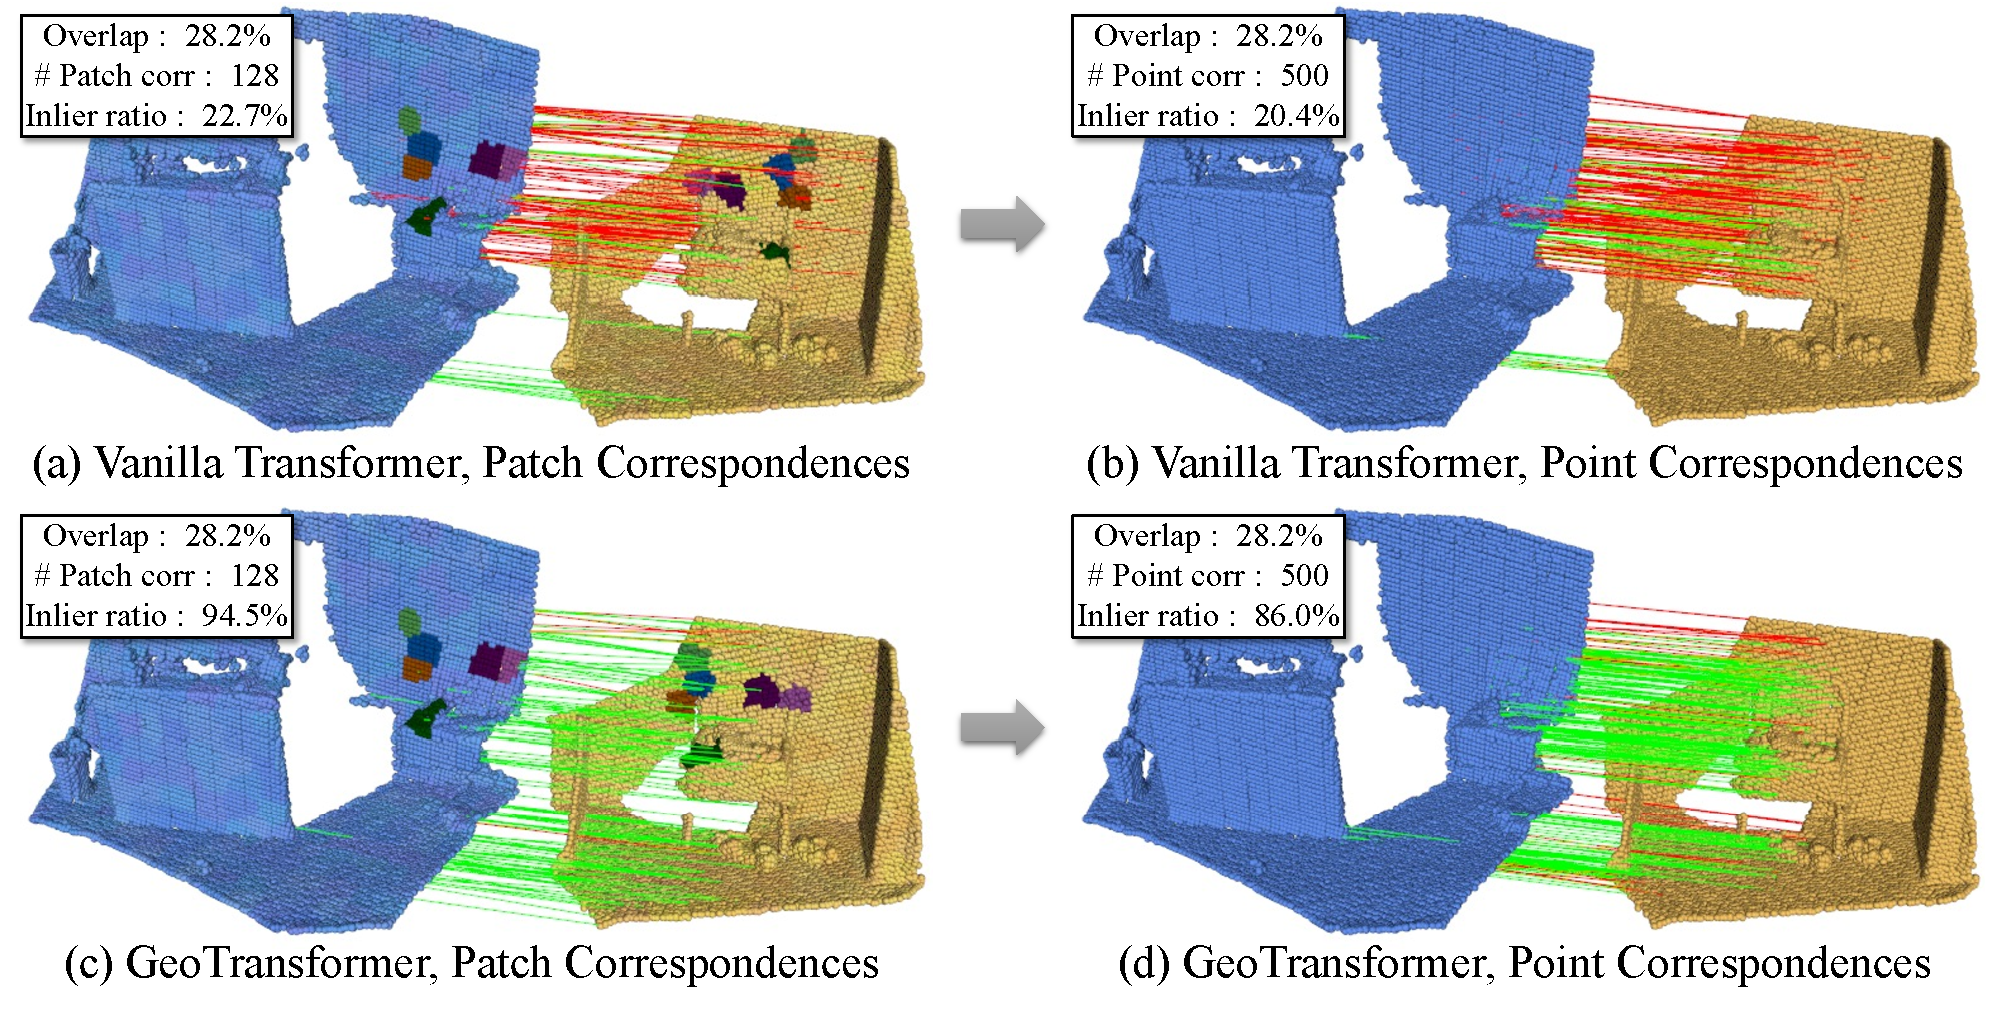
\includegraphics[width=\textwidth]{images/teaser.pdf}
    \caption{\textbf{多实例点云配准: } 给定目标的模板点云,成对点云配准(左)侧重于估计模板点云和目标点云之间的单个刚性变换,而多实例点云配准(右)旨在估计目标点云中相同物体的6D位姿。
    }
    \label{fig:teaser}
    \vspace{-10mm}
\end{figure*}

目前大多数点云配准任务研究主要集中在成对配准上。然而,在实际应用中,目标场景可能包含多个重复实例,我们需要估计模板点云与目标点云中这些重复实例之间的多个刚性变换。比如说在室内场景中,我们希望机器人能够将屋子中所有的椅子摆正,那么首先需要将多个椅子点云和模板椅子点云进行配准,求的目标椅子的位姿,通过机械运动来达到位姿改变的效果。图 \ref{fig:teaser} 展示了了一个示例。这个问题被命名为多实例点云配准,它比成对点云配准更具挑战性。针对该任务已有的现有文献研究较少,扩展现有的点云配准方法来解决这个问题并非易事。多实例点云配准不仅需要从嘈杂的对应中拒绝异常值,还需要识别单个实例的异常值集,这使得它比传统的配准问题更具挑战性。

与传统的两两配准方法相比,多实例点云配准需要解决更复杂的问题,同时也具有更广泛的应用价值。比如,在大规模场景重建任务中,通常需要处理成千上万个点云数据。单纯采用两两配准的方法可能导致累积误差,从而影响重建结果的精度。因此,研究多实例点云配准算法具有重要的实际意义。在机械臂抓取任务中,多实例点云配准算法可以在全局范围内考虑点云之间的约束关系,有助于消除局部误差和噪声的影响,从而提高配准结果的鲁棒性 \cite{stuckler2012robust} 。

尽管多实例点云配准技术在近年来取得了显著的进展,仍然存在许多亟待解决的问题。例如,现存的多实例点云配准一般采用多任务的方式,也就是先对点云分割或者三维目标检测,然后进行两两点云配准,这样的方式需要先训练点云分割或者目标检测网络,泛化性差。并且如果见到了不存在先验的点云,下游的配准任务仍然会失效。所以,本文我们会对多实例点云配准进行研究,通过点云直接进行多实例点云配准,不需要先进行点云分割或者目标检测,从而提高多实例点云配准的泛化性。


\section{国内外研究现状}

\subsection{点云配准}
点云配准长期以来一直是计算机视觉和机器人领域的一项基本任务,大致可分为直接方法 \cite{besl1992method, pomerleau2015review} 和基于特征的方法 \cite{qi2017pointnet,huang2021predator,bai2021pointdsc} 。近年来,由于深度学习的发展,许多基于特征的方法取得了最先进的性能。这些方法通常通过特征匹配产生对应关系,然后移除异常值以稳健地估计转换。尽管深度特征 \cite{qi2017pointnet,huang2021predator,bai2021pointdsc, wang2022you} 发展迅速,但特征匹配生成的对应关系仍然包含异常值。因此,去除异常点在点云配准中具有重要意义。过去,已经提出了许多传统方法来去除异常值,包括基于RANSAC的方法 \cite{barath2021progressive,zhao2021progressive,barath2018graph} 、基于分支和边界的方法 \cite{kluger2020consac} 以及许多其他方法 \cite{huang2021predator,yang2020teaser} 。最近,一系列基于学习的方法 \cite{bai2020d3feat,yi2018learning} 被提出,并在异常值去除方面取得了显着的效果。
以上的方法都是基于成对点云配准来完成的。然而,与成对配准不同,一个实例的内点构成多实例点云配准中所有其他实例的异常值。这种伪异常值使得很难将上述二元分类模型直接推广到多实例点云配准的情况。
现有该问题解决方案包括采用目标检测方法或对目标点云应用实例分割,将多实例点云配准问题转化为多个成对点云配准问题,但是这种方法需要预先训练一个目标检测或者点云分割网络,这样的方法对于已有点云类别是有效的,但是对于未知的类别是不适用的。另一种解决方案是通过多模型拟合,但是现有的多模型拟合方法依赖于抽样有效假设,当模型数量或离群率变高时,会涉及大量的抽样步骤,使得这些算法的效率和鲁棒性急剧下降。

\subsection{三维目标检测和实例分割}
三维物体的目标检测和实例分割与多实例点云配准有着密切的关系。输入一帧点云,目标检测模型 \cite{qi2019deep} 可以用来对获取每个目标对象的边界框,三维实例分割 \cite{wang2018sgpn,han2020occuseg} 为每个点生成实例标签。

这样的方法产生的结果类似于多实例点云配准的结果,但是它们需要将特定对象或类别的先验训练到网络中。基于点云匹配的筛选和聚类方法来进行多实例点云配准通过直接将模板点云和目标点云中的多个实例对齐来处理两组点云,而不使用任何关于输入的点云的先验信息。

\subsection{多模型拟合}
多实例配准也可以通过多模型拟合来实现,其目的是根据多个模型生成的数据点来进行建模。例如在点云中拟合多个平面 \cite{barath2018multi} ,在运动分割中估计基本矩阵 \cite{hartley1997defense} ,在多实例点云配准中计算刚性变换 \cite{tang2022multi} 等。但是由于一个实例的正常值构成所有其他实例的离群值,所以多模型拟合比单模型拟合更具挑战性。

现有的多模型拟合方法大致可以分为两类。第一类按顺序拟合模型 \cite{barath2019progressive,barath2021progressive,kanazawa2004detection,kluger2020consac} ,通过重复采样和筛选模型来进行建模。比如,Progressive-X \cite{barath2019progressive} 和Progressive-X+ \cite{barath2021progressive} 使用了表现更好的Graph-cut RANSAC \cite{barath2018graph} 作为采样方法来生成假设。CONSAC \cite{kluger2020consac} 首次将深度模型引入多模型拟合中,使用类似PointNet \cite{qi2017pointnet} 的网络来引导采样。通过重复采样来恢复单个实例,从输入中删除正常值和,以顺序的方式来检测实例。

第二类模型同时拟合多个模型 \cite{tang2022multi,toldo2008robust,magri2016multiple,magri2014t,magri2015robust} 。许多基于偏好分析的方法 \cite{toldo2008robust,magri2015robust} 最初对一系列假设进行采样,然后根据假设的残差对输入点进行聚类。ECC \cite{tang2022multi} 利用点云刚性变换空间一致性 \cite{leordeanu2005spectral} 和以自下而上的方式基于距离不变矩阵对对应关系进行聚类。PointCLM \cite{yuan2022pointclm} 使用了一种新的深层表示方法来与空间一致性相结合,得到了更好的结果。

% 本项目希望基于旋转等变的描述子来实现性能的初步提升,希望在模型中加入更多的内在形状和几何信息。通过端到端的方法优化整个方法系统,实现更高的准确性和鲁棒性。
\section{论文结构安排}
本论文共分为6章。

第一章为绪论,本章主要阐述了三维点云配准研究的重要性、背景以及现有的研究进展。通过对国内外三维点云配准研究文献的梳理和调查,我们对该领域的发展轨迹和现状进行了总结,并分析了先前研究所展现出的优点与缺点。同时,我们也详细介绍了本研究所完成的主要任务和做出的关键贡献。考虑到过去的研究中仍存在未完全解决的问题和挑战,我们特别指出了本研究所应用的策略和解决方案。最后,我们规划了清晰的文章结构,以引导读者理解本研究的整体框架。

在第二章,我们主要阐述了三维点云的基本数据格式和在本研究中所涉及的基础数学知识。同时,我们对在本研究中所用到的关于三维刚体变换的基础知识进行了详尽的总结和描述。

第三章在介绍了主要的数据集和评价指标后,引出深度学习方法在三维点云配准领域的研究与应用,并结合深度学习在三维点云配准领域做出的代表性工作 PointNet \cite{qi2017pointnet} 和 PointNet++ \cite{qi2017pointnet++} 进行介绍,并介绍和使用 PREDATOR \cite{huang2021predator} 作为骨干网络提取点云的点对特征供后续使用。

第四章主要介绍了本文提出的多实例点云配准,首先我们根据点云的特征进行聚类,然后对每个聚类进行对应聚类,最后进行刚性变换估计;其次,我们引入深度学习的方法,学习鲁棒的点对特征,进行谱聚类,得到了点云配准更好的效果和更高的指标。

第五章主要介绍了本文的实验结果,包括多实例点云配准的定性和定量实验,证明了本文提出的方法的有效性和鲁棒性。
\section{小结}
本章主要介绍了点云配准任务以及多实例点云配准任务的研究背景和研究意义、国内外研究现状。然后介绍了本文的研究内容和结构安排。

%%
% The BIThesis Template for Bachelor Paper Translation
%
% 北京理工大学毕业设计(论文) —— 使用 XeLaTeX 编译
%
% Copyright 2020-2023 BITNP
%
% This work may be distributed and/or modified under the
% conditions of the LaTeX Project Public License, either version 1.3
% of this license or (at your option) any later version.
% The latest version of this license is in
%   http://www.latex-project.org/lppl.txt
% and version 1.3 or later is part of all distributions of LaTeX
% version 2005/12/01 or later.
%
% This work has the LPPL maintenance status `maintained'.
%
% The Current Maintainer of this work is Feng Kaiyu.
%
% Compile with: xelatex -> biber -> xelatex -> xelatex
%%

% 第一章节

\chapter{相关工作}
\label{sec:related}

\section{基于对应关系的方法。}
我们的工作遵循基于对应关系的方法的思路~\cite{deng2018ppfnet,deng2018ppf,gojcic2019perfect,choy2019fully}。
它们首先提取两个点云之间的对应关系,然后使用稳健的姿态估计器,例如RANSAC,恢复变换。
由于稳健的估计器,它们在室内和室外场景配准中取得了最新的性能。
这些方法可以根据它们提取对应关系的方式进一步分类为两类。
第一类旨在检测更可重复的关键点~\cite{bai2020d3feat,huang2021predator}并为关键点学习更强大的描述符~\cite{choy2019fully,ao2021spinnet,wang2021you}。
而第二类~\cite{yu2021cofinet}通过考虑所有可能的匹配而不需要检测关键点来检索对应关系。
我们的方法遵循无需检测的方法,并通过利用几何信息来提高对应关系的准确性。

\section{直接配准方法。}
最近,直接配准方法已经出现。他们以端到端的方式使用神经网络估计变换。
这些方法可以进一步分为两类。
第一类~\cite{wang2019deep,wang2019prnet,yew2020rpm,fu2021robust}遵循ICP~\cite{besl1992method}的思路,该方法迭代地建立软对应关系,并使用可微分的加权SVD计算变换。
第二类~\cite{aoki2019pointnetlk,huang2020feature,xu2021omnet}首先为每个点云提取一个全局特征向量,并使用全局特征向量回归变换。
虽然直接配准方法在单个合成形状上取得了有希望的结果,但在大规模场景中它们可能会失败,如~\cite{huang2021predator}所述。

\section{深度稳健估计器。}
由于传统的稳健估计器,如RANSAC在高离群值比率的情况下会出现收敛速度慢和不稳定的问题,因此提出了深度稳健估计器~\cite{pais20203dregnet,choy2020deep,bai2021pointdsc}作为替代方案。
它们通常包含一个分类网络来拒绝离群值和一个估计网络来计算变换。
与传统的稳健估计器相比,它们在准确性和速度上都有所改进。
然而,它们需要训练一个特定的网络。
相比之下,我们的方法通过一个无参数的局部到全局的配准方案实现了快速和精确的配准。
%%
% The BIThesis Template for Bachelor Paper Translation
%
% 北京理工大学毕业设计(论文) —— 使用 XeLaTeX 编译
%
% Copyright 2020-2023 BITNP
%
% This work may be distributed and/or modified under the
% conditions of the LaTeX Project Public License, either version 1.3
% of this license or (at your option) any later version.
% The latest version of this license is in
%   http://www.latex-project.org/lppl.txt
% and version 1.3 or later is part of all distributions of LaTeX
% version 2005/12/01 or later.
%
% This work has the LPPL maintenance status `maintained'.
%
% The Current Maintainer of this work is Feng Kaiyu.
%
% Compile with: xelatex -> biber -> xelatex -> xelatex
%%

% 第一章节

\chapter{方法}
\label{sec:geotrans}

%!TEX root = ../geotrans.tex

\begin{figure*}[t]
  \begin{overpic}[width=1.0\linewidth]{figures/images/pipeline.pdf}
  \put(0,40.3){\scriptsize \rule[-0.4ex]{0.2ex}{1.0em}\rule[0.6ex]{2.2ex}{0.1em} 1. Feature Extraction \rule[0.6ex]{2.2ex}{0.1em}\rule[-0.4ex]{0.2ex}{1.0em}}
  \put(15.55,40.3){\scriptsize \rule[-0.4ex]{0.2ex}{1.0em}\rule[0.6ex]{6ex}{0.1em} 2. Superpoint Matching \rule[0.6ex]{6ex}{0.1em}\rule[-0.4ex]{0.2ex}{1.0em}}
  \put(37.4,40.3){\scriptsize \rule[-0.4ex]{0.2ex}{1.0em}\rule[0.6ex]{13.2ex}{0.1em} 3. Point Matching \rule[0.6ex]{13.2ex}{0.1em}\rule[-0.4ex]{0.2ex}{1.0em}}
  \put(65.2,40.3){\scriptsize \rule[-0.4ex]{0.2ex}{1.0em}\rule[0.6ex]{12.7ex}{0.1em} 4. Local-to-Global Registration \rule[0.6ex]{12.7ex}{0.1em}\rule[-0.4ex]{0.2ex}{1.0em}}
  \end{overpic}
  \vspace{-20pt}
  \caption{The backbone downsamples the input point clouds and learns features in multiple resolution levels. The Superpoint Matching Module extracts high-quality superpoint correspondences between $\hat{\mathcal{P}}$ and $\hat{\mathcal{Q}}$ using the Geometric Transformer which iteratively encodes intra-point-cloud geometric structures and inter-point-cloud geometric consistency. The superpoint correspondences are then propagated to dense points $\tilde{\mathcal{P}}$ and $\tilde{\mathcal{Q}}$ by the Point Matching Module. Finally, the transformation is computed with a local-to-global registration method.}
  \label{fig:overview}
  \vspace{-10pt}
\end{figure*}


给定两个点云$\mathcal{P} = \{\textbf{p}_i \in \mathbb{R}^3 \mid i = 1, ..., N\}$ 和 $\mathcal{Q} = \{\textbf{q}_i \in \mathbb{R}^3 \mid i = 1, ..., M\}$,我们的目标是估计一个刚性变换$\textbf{T} = \{\textbf{R}, \textbf{t}\}$来对齐这两个点云,其中$\textbf{R} \in SO(3)$是3D旋转,$\textbf{t} \in \mathbb{R}^3$是3D平移。变换可以通过以下方式求解:
% \vspace{-3pt}
\begin{equation}
\min_{\textbf{R}, \textbf{t}} \sum\nolimits_{(\textbf{p}^{*}_{x_i}, \textbf{q}^{*}_{y_i}) \in \mathcal{C}^{*}} \lVert \textbf{R} \cdot \textbf{p}^{*}_{x_i} + \textbf{t} - \textbf{q}^{*}_{y_i} \rVert^2_2.
% \vspace{-3pt}
\end{equation}
在这里,$\mathcal{C}^{*}$是$\mathcal{P}$和$\mathcal{Q}$之间的真实对应关系集合。由于在实际中我们无法知道$\mathcal{C}^{*}$,所以我们需要首先在两个点云之间建立点对应关系,然后估计对齐变换。

我们的方法采用分层对应关系模式,以从粗到细的方式找到对应关系。我们采用KPConv-FPN同时对输入点云进行下采样并提取点特征(\ref{sec:model-backbone})。第一级和最后一级(最粗糙的)下采样点对应于需要匹配的密集点和超点。使用\emph{超点匹配模块}提取超点对应关系,其相邻的局部区域与彼此重叠(\ref{sec:model-pam})。基于此,\emph{点匹配模块}进一步将超点对应关系细化到密集点(\ref{sec:model-pom})。最后,从密集对应关系中恢复对齐变换,无需依赖RANSAC(\ref{sec:model-estimation})。流程图示在\ref{fig:overview}中。

\section{超点采样和特征提取}
\label{sec:model-backbone}
我们利用KPConv-FPN主干~\cite{thomas2019kpconv,lin2017feature}为点云提取多级特征。点特征学习的一个副产品是点下采样。我们在下采样点上进行工作,因为点云配准实际上可以通过一组更粗糙的点的对应关系来确定。原始点云通常过于密集,以至于点对点的对应关系是多余的,有时甚至过于集中而无法使用。

对应于最粗糙的分辨率的点,由$\hat{\mathcal{P}}$和$\hat{\mathcal{Q}}$表示,被视为需要匹配的\emph{超点}。相关的学习特征被表示为$\hat{\textbf{F}}{}^{\mathcal{P}} {\in} \mathbb{R}^{\lvert \hat{\mathcal{P}} \rvert \times \hat{d}}$ 和 $\hat{\textbf{F}}{}^{\mathcal{Q}} {\in} \mathbb{R}^{\lvert \hat{\mathcal{Q}} \rvert \times \hat{d}}$。
在原始分辨率的$1/2$处计算密集点对应关系,即,由$\tilde{\mathcal{P}}$ 和 $\tilde{\mathcal{Q}}$表示的第一级下采样点。他们的学习特征由$\tilde{\textbf{F}}{}^{\mathcal{P}} {\in} \mathbb{R}^{\lvert \tilde{\mathcal{P}} \rvert \times \tilde{d}}$ 和 $\tilde{\textbf{F}}{}^{\mathcal{Q}} {\in} \mathbb{R}^{\lvert \tilde{\mathcal{Q}} \rvert \times \tilde{d}}$表示。

对于每个超点,我们使用点到节点分组策略 \cite{li2018so,yu2021cofinet}在其周围构建一个局部\emph{贴片}。
特别地,$\tilde{\mathcal{P}}$中的每个点及其来自$\tilde{\textbf{F}}{}^{\mathcal{P}}$的特征都分配给几何空间中最近的超点:
\vspace{-2pt}
\begin{equation}
\mathcal{G}^{\mathcal{P}}_i = \{\tilde{\textbf{p}} \in \tilde{\mathcal{P}} \mid i = \arg\min\nolimits_j (\lVert \tilde{\textbf{p}} - \hat{\textbf{p}}_j \rVert_2), \hat{\textbf{p}}_j \in \hat{\mathcal{P}}\}.
\vspace{-2pt}
\end{equation}
这本质上导致了由超点生成的输入点云的Voronoi分解。
与$\mathcal{G}^{\mathcal{P}}_i$中的点相关的特征矩阵表示为$\textbf{F}^{\mathcal{P}}_i \subset \tilde{\textbf{F}}{}^{\mathcal{P}}$。
具有空贴片的超点将被移除。
对于$\mathcal{Q}$,计算并以类似方式表示贴片$\{\mathcal{G}^{\mathcal{Q}}_i\}$和特征矩阵$\{\textbf{F}^{\mathcal{Q}}_i\}$。

\section{超点匹配模块}
\label{sec:model-pam}
%在粗到细的匹配流程中,点对应关系的准确性大大受到超点(贴片)匹配准确性的影响。我们设计了一种新颖的变换器模块,以实现高度可靠的超点匹配。

%!TEX root = ../geotrans.tex

\begin{figure}[t]
  \centering
  \begin{overpic}[width=1.0\linewidth]{figures/images/geo-self-att.pdf}
  \end{overpic}
  \vspace{-20pt}
  \caption{Left: The structure of geometric self-attention module. Right: The computation graph of geometric self-attention.}
  \label{fig:geotr}
  \vspace{-10pt}
\end{figure}


%\vspace{-10pt}
\subsection{Geometric Transformer.}
%
全局上下文在许多计算机视觉任务中已被证明至关重要~\cite{dosovitskiy2020image,sun2021loftr,yu2021cofinet}。
因此,Transformer被用来利用全局上下文信息进行点云配准。
然而,现有的方法~\cite{wang2019deep,huang2021predator,yu2021cofinet}通常只将高级点云特征提供给变换器,并不明确地编码几何结构。
这使得学习到的特征在几何上的区分度较低,导致严重的匹配模糊和大量的异常匹配,特别是在重叠度低的情况下。
一种直接的解决方案是明确注入3D点坐标的位置嵌入~\cite{yang2019modeling,zhao2021point}。
然而,由此产生的基于坐标的变换器自然是\emph{变换变化的},而配准需要\emph{变换不变性},因为输入点云可以处于任意姿态。

为此,我们提出了\emph{Geometric Transformer},它不仅编码高级点特征,而且明确捕捉点云内部的几何结构和点云间的几何一致性。
GeoTransformer由一个\emph{几何自注意}模块组成,用于学习点云内部特征,以及一个\emph{基于特征的交叉注意}模块,用于建模点云间的一致性。这两个模块交错进行$N_t$次,以提取混合特征$\hat{\textbf{H}}^{\mathcal{P}}$和$\hat{\textbf{H}}^{\mathcal{Q}}$,用于可靠的超点匹配(见\ref{fig:overview}(左下角))。

\subsection{几何自注意力.}
%
我们设计了一个\emph{几何自注意力}机制,以学习每个点云中超点在特征和几何空间中的全局关联性。以下,我们描述了对$\hat{\mathcal{P}}$的计算,对$\hat{\mathcal{Q}}$的计算也是相同的。给定输入特征矩阵$\textbf{X} \in \mathbb{R}^{\lvert \hat{\mathcal{P}} \vert \times d_t}$,输出特征矩阵$\textbf{Z} \in \mathbb{R}^{\lvert \hat{\mathcal{P}} \vert \times d_t}$是所有投影输入特征的加权和:
\vspace{-5pt}
\begin{equation}
\textbf{z}_i = \sum_{j=1}^{\lvert \hat{\mathcal{P}} \vert} a_{i, j} (\textbf{x}_j\textbf{W}^V),
\vspace{-5pt}
\end{equation}
其中,权重系数$a_{i, j}$是对注意力得分$e_{i, j}$进行行方向的softmax计算得到的,$e_{i, j}$计算如下:
\vspace{-5pt}
\begin{equation}
e_{i, j} = \frac{(\textbf{x}_i\textbf{W}^Q)(\textbf{x}_j\textbf{W}^K + \textbf{r}_{i, j}\textbf{W}^R)^T}{\sqrt{d_{t}}}.
\vspace{-5pt}
\end{equation}
这里,$\textbf{r}_{i, j} \in \mathbb{R}^{d_t}$是一个将在下文描述的\emph{几何结构嵌入}。$\textbf{W}^Q, \textbf{W}^K, \textbf{W}^V, \textbf{W}^R \in \mathbb{R}^{d_t \times d_t}$分别是查询、键、值和几何结构嵌入的投影矩阵。\ref{fig:geotr}显示了几何自注意力的结构和计算。

我们设计了一种新颖的\emph{几何结构嵌入},用来编码超点的变换不变的几何结构。核心思想是利用与超点计算的距离和角度,这些是在同一场景的不同点云中保持一致的。给定两个超点$\hat{\textbf{p}}_i, \hat{\textbf{p}}_j \in \hat{\mathcal{P}}$,它们的几何结构嵌入由一个\emph{成对距离嵌入}和一个\emph{三元角嵌入}组成,这些将在下面详细描述。

(1) \emph{成对距离嵌入}.
给定$\hat{\textbf{p}}_i$和$\hat{\textbf{p}}_j$之间的距离$\rho_{i, j} \hspace{1pt} {=} \hspace{1pt} \lVert \hat{\textbf{p}}_i - \hat{\textbf{p}}_j \rVert_2$,它们之间的距离嵌入$\textbf{r}^D_{i, j}$通过对$\rho_{i, j} / \sigma_d$应用正弦函数 \cite{vaswani2017attention}来计算。这里,$\sigma_d$是一个超参数,用来调整对距离变化的敏感性。

(2) \emph{三元角嵌入}.
我们用超点的三元组计算角嵌入。首先,我们选择$\hat{\textbf{p}}_i$的$k$个最近邻点$\mathcal{K}_i$。对于每个$\hat{\textbf{p}}_x \in \mathcal{K}_i$,我们计算角度$\alpha^x_{i,j} = \angle(\Delta_{x, i}, \Delta_{j, i})$,其中$\Delta_{i, j} := \hat{\textbf{p}}_i - \hat{\textbf{p}}_j$。然后,三元角嵌入$\textbf{r}^A_{i, j, x}$通过对$\alpha^x_{i,j} / \sigma_a$应用正弦函数来计算,其中$\sigma_a$控制对角度变化的敏感性。

最后,通过聚合成对距离嵌入和三元角嵌入来计算几何结构嵌入$\textbf{r}_{i, j}$:
\vspace{-5pt}
\begin{equation}
\textbf{r}_{i, j} = \textbf{r}^D_{i, j}\textbf{W}^D + {\max}_x\left\{\textbf{r}^A_{i, j, x}\textbf{W}^A\right\},
\vspace{-5pt}
\label{eq:gse}
\end{equation}
其中,$\textbf{W}^D, \textbf{W}^A \in \mathbb{R}^{d_t \times d_t}$分别是两种嵌入的投影矩阵。我们在这里使用最大池化来提高对由于自遮挡而导致的超点的不同最近邻的鲁棒性。\ref{fig:rge}显示了几何结构嵌入的计算。

%!TEX root = ../geotrans.tex

\begin{figure}[t]
  \begin{overpic}[width=1.0\linewidth]{figures/images/geo-emb.pdf}
  \end{overpic}
  \vspace{-20pt}
  \caption{An illustration of the distance-and-angle-based geometric structure encoding and its computation.}
  \label{fig:rge}
  \vspace{-10pt}
\end{figure}


% \vspace{-10pt}
\subsection{基于特征的交叉注意力.}
%
交叉注意力是点云配准任务的典型模块~\cite{huang2021predator,wang2019deep,yu2021cofinet},用于在两个输入点云之间进行特征交换。
给定$\hat{\mathcal{P}}$,$\hat{\mathcal{Q}}$的自注意力特征矩阵$\textbf{X}^{\mathcal{P}}$,$\textbf{X}^{\mathcal{Q}}$,$\hat{\mathcal{P}}$的交叉注意力特征矩阵$\textbf{Z}^{\mathcal{P}}$使用$\hat{\mathcal{Q}}$的特征计算:
\vspace{-2pt}
\begin{equation}
\textbf{z}^{\mathcal{P}}_i = \sum_{j=1}^{\lvert \hat{\mathcal{Q}} \rvert} a_{i, j} (\textbf{x}^{\mathcal{Q}}_j\textbf{W}^V).
\vspace{-2pt}
\end{equation}
同样,$a_{i, j}$是对交叉注意力得分$e_{i, j}$进行行方向的softmax计算,而$e_{i, j}$是$\textbf{X}^{\mathcal{P}}$和$\textbf{X}^{\mathcal{Q}}$之间的特征相关性计算:
\vspace{-2pt}
\begin{equation}
e_{i, j} = \frac{(\textbf{x}^{\mathcal{P}}_i\textbf{W}^Q)(\textbf{x}^{\mathcal{Q}}_j\textbf{W}^K)^T}{\sqrt{d_{t}}}.
\vspace{-2pt}
\end{equation}
$\mathcal{Q}$的交叉注意力特征以相同的方式计算。
虽然几何自注意力模块为每个单独的点云编码了变换不变的几何结构,基于特征的交叉注意力模块可以在两个点云之间建模几何一致性。
所得到的混合特征既不变于变换,又对推理对应关系具有鲁棒性。

% \vspace{-10pt}
\subsection{超点匹配.}
%
为了找到超点的对应关系,我们提出了一种基于全局特征相关性的匹配方案。
我们首先将$\hat{\textbf{H}}{}^{\mathcal{P}}$和$\hat{\textbf{H}}{}^{\mathcal{Q}}$归一化到单位超球面,并计算一个高斯相关矩阵$\textbf{S} \in \mathbb{R}^{\lvert \hat{\mathcal{P}} \rvert \times \lvert \hat{\mathcal{Q}} \rvert}$,其中$s_{i, j} = \exp(-\lVert \hat{\textbf{h}}{}^{\mathcal{P}}_i - \hat{\textbf{h}}{}^{\mathcal{Q}}_j\rVert_2^2)$。
在实践中,点云的一些区域在几何上较不具有区分性,并且在另一个点云中有许多相似的区域。除了我们强大的混合特征外,我们还对$\textbf{S}$进行双向归一化操作 \cite{rocco2018neighbourhood,sun2021loftr},进一步抑制模糊的匹配,得到$\bar{\textbf{S}}$:
\vspace{-2pt}
\begin{equation}
\bar{s}_{i, j} = \frac{s_{i, j}}{\sum_{k=1}^{\lvert \hat{\mathcal{Q}} \rvert} s_{i, k}} \cdot \frac{s_{i, j}}{\sum_{k=1}^{\lvert \hat{\mathcal{P}} \rvert} s_{k, j}}.
\vspace{-2pt}
\end{equation}
我们发现这种抑制可以有效地消除错误的匹配。
最后,我们选择$\bar{\textbf{S}}$中最大的$N_{c}$个项作为\emph{超点对应关系}:
% \vspace{-2pt}
\begin{equation}
\hat{\mathcal{C}} = \{ (\hat{\textbf{p}}_{x_i}, \hat{\textbf{q}}_{y_i}) \mid (x_i, y_i) \in \mathrm{topk}_{x, y}(\bar{s}_{x, y}) \}.
% \vspace{-2pt}
\end{equation}
由于GeoTransformer的强大几何结构编码能力,我们的方法能够在低重叠情况和少量点对应关系下,最显著的是,以一种无需RANSAC的方式实现准确的配准。

\subsection{点匹配模块}
\label{sec:model-pom}

得到超点对应关系后,我们使用一个简单而有效的\emph{点匹配模块}来提取点对应关系。
在点级别,我们只使用由骨干网络学习的局部点特征。
其原理是,一旦通过超点匹配解决了全局的模糊性,点级别的匹配主要由两个匹配点的邻域决定。
这种设计选择提高了鲁棒性。

对于每个超点对应关系$\hat{\mathcal{C}}_i = (\hat{\textbf{p}}_{x_i}, \hat{\textbf{q}}_{y_i})$,我们使用一个最优传输层 \cite{sarlin2020superglue} 来提取$\mathcal{G}^{\mathcal{P}}_{x_i}$和$\mathcal{G}^{\mathcal{Q}}_{y_i}$之间的\emph{局部稠密点对应关系}。
具体来说,我们首先计算一个成本矩阵$\textbf{C}_i \in \mathbb{R}^{n_i \times m_i}$:
\vspace{-2pt}
\begin{equation}
\textbf{C}_i = \textbf{F}^{\mathcal{P}}_{x_i} (\textbf{F}^{\mathcal{Q}}_{y_i})^T / \sqrt{\tilde{d}},
\vspace{-2pt}
\end{equation}
其中$n_i = \lvert \mathcal{G}^{\mathcal{P}}_{x_i} \rvert$,$m_i = \lvert \mathcal{G}^{\mathcal{Q}}_{y_i} \rvert$。
然后,我们将成本矩阵$\textbf{C}_i$通过追加一个新行和一个新列扩增为$\bar{\textbf{C}}_i$,新行和新列的值由一个可学习的垃圾箱参数$\alpha$填充,如文献 \cite{sarlin2020superglue} 中所述。
然后我们利用Sinkhorn算法 \cite{sinkhorn1967concerning} 在$\bar{\textbf{C}}_i$上计算一个软分配矩阵$\bar{\textbf{Z}}_i$,然后通过丢弃最后一行和最后一列恢复为$\textbf{Z}_i$。
我们使用$\textbf{Z}_i$作为候选匹配的置信度矩阵,并通过互相选择前$k$个进行点对应关系的提取,其中,如果一个点匹配位于它所在的行和列的$k$个最大项中,则选择该点匹配:
\vspace{-2pt}
\begin{equation}
\mathcal{C}_i = \{(\mathcal{G}^{\mathcal{P}}_{x_i}(x_j), \mathcal{G}^{\mathcal{Q}}_{y_i}(y_j)) \mid (x_j, y_j) \in \mathrm{mutual\_topk}_{x, y}(z^i_{x, y})\}.
% \vspace{-5pt}
\end{equation}
然后将每个超点匹配计算出的点对应关系收集到一起,形成最终的\emph{全局稠密点对应关系}:$\mathcal{C} = \bigcup_{i=1}^{N_c} \mathcal{C}_i$。

\subsection{无需RANSAC的局部到全局配准}
\label{sec:model-estimation}

先前的方法通常依赖于稳健的姿态估计器来估计变换,因为假定的对应关系常常被离群值主导。
大多数稳健估计器,如RANSAC,收敛速度较慢。
鉴于GeoTransformer的高内点比例,我们能够实现稳健的配准,而无需依赖稳健估计器,这也大大降低了计算成本。

我们设计了一个\emph{局部到全局配准}(LGR)方案。
作为一种假设验证方法,LGR包括一个局部阶段的变换候选生成和一个全局阶段的变换选择。
在局部阶段,我们使用其\emph{局部点对应关系}为每个超点匹配求解一个变换$\textbf{T}_i = \{\textbf{R}_i, \textbf{t}_i\}$:
\vspace{-2pt}
\begin{equation}
\textbf{R}_i, \textbf{t}_i = \min_{\textbf{R}, \textbf{t}} \sum\nolimits_{(\tilde{\textbf{p}}_{x_j}, \tilde{\textbf{q}}_{y_j}) \in \mathcal{C}_i} w^i_j \lVert \textbf{R} \cdot \tilde{\textbf{p}}_{x_j} \hspace{-3pt} + \textbf{t} - \tilde{\textbf{q}}_{y_j} \rVert_2^2.
\label{eq:weighted-svd}
\vspace{-2pt}
\end{equation}
这可以使用加权SVD~\cite{besl1992method}以闭式解决。
$\textbf{Z}_i$中每个对应关系的相应置信度得分用作权重$w^i_j$。
由于对应关系的高质量,这个阶段获得的变换已经非常准确。
在全局阶段,我们选择在整个\emph{全局点对应关系}中接受最多内点匹配的变换:
\vspace{-2pt}
\begin{equation}
\textbf{R}, \textbf{t} = \max_{\textbf{R}_i, \textbf{t}_i} \sum\nolimits_{(\tilde{\textbf{p}}_{x_j}, \tilde{\textbf{q}}_{y_j}) \in \mathcal{C}} \llbracket \lVert \textbf{R}_i \cdot \tilde{\textbf{p}}_{x_j} \hspace{-3pt} + \textbf{t}_i - \tilde{\textbf{q}}_{y_j} \rVert_2^2 < \tau_a \rrbracket,
\end{equation}
其中$\llbracket \cdot \rrbracket$是Iverson括号。$\tau_a$是接受半径。
然后,我们通过求解\ref{eq:weighted-svd},迭代地使用存活的内点匹配重新估计变换$N_r$次。
如\ref{sec:exp-indoor}所示,我们的方法在RANSAC的配准精度上实现了可比较的结果,但将计算时间减少了100倍以上。
此外,与深度稳健估计器~\cite{choy2020deep,pais20203dregnet,bai2021pointdsc}不同,我们的方法是无参数的,不需要网络训练。

\subsection{损失函数}
\label{sec:model-loss}

损失函数$\mathcal{L} = \mathcal{L}_{oc} + \mathcal{L}_{p}$由用于超点匹配的\emph{重叠感知圆形损失} $\mathcal{L}_{oc}$和用于点匹配的\emph{点匹配损失} $\mathcal{L}_{p}$组成。

% \vspace{-10pt}
\textbf{重叠感知圆形损失。}
%
现有的方法~\cite{sun2021loftr,yu2021cofinet}通常将超点匹配形式化为多标签分类问题,并采用带双重softmax~\cite{sun2021loftr}或最优传输~\cite{sarlin2020superglue,yu2021cofinet}的交叉熵损失。
每个超点被分配(分类)给一个或多个其他超点,其中基于patch重叠计算的ground truth,很可能一个patch会与多个patch重叠。
通过分析交叉熵损失的梯度,我们发现在多标签分类中,具有高置信度得分的正类被正梯度抑制。
这阻碍了模型从中提取可靠的超点对应关系。

为了解决这个问题,我们选择以度量学习的方式提取超点描述符。
一个直接的解决方案是采用类似于~\cite{bai2020d3feat,huang2021predator}的圆形损失~\cite{sun2020circle}。
然而,圆形损失忽视了正样本之间的差异,并对它们进行了等权重的处理。
因此,它在匹配重叠相对较低的patch时遇到困难。
出于这个原因,我们设计了一个\emph{重叠感知的圆形损失},以使模型关注那些重叠较高的匹配。
我们选择在$\mathcal{Q}$中至少有一个正patch的$\mathcal{P}$中的patch,以形成一组锚定patch,$\mathcal{A}$。
如果一对patch至少有$10\%$的重叠,那么它们是正的,如果它们没有重叠,那么它们是负的。
所有其他对都被忽略。
对于每个锚定patch $\mathcal{G}^{\mathcal{P}}_i \in \mathcal{A}$,我们将其在$\mathcal{Q}$中的正patch集合表示为$\varepsilon^i_p$,其负patch集合表示为$\varepsilon^i_n$。
然后在$\mathcal{P}$上定义重叠感知的圆形损失为:
\begin{equation}
\label{eq:overlap-aware-circle-loss}
\mathcal{L}^{\mathcal{P}}_{oc} = \frac{1}{\lvert\mathcal{A}\rvert} \sum_{\mathclap{\mathcal{G}^{\mathcal{P}}_i \in \mathcal{A}}} \log[1 + \sum_{\mathclap{\mathcal{G}^{\mathcal{Q}}_j \in \varepsilon^i_p}} e^{\lambda^j_i\beta^{i,j}_p (d^j_i - \Delta_p)} \cdot \sum_{\mathclap{\mathcal{G}^{\mathcal{Q}}_k \in \varepsilon^i_n}} e^{\beta^{i,k}_n (\Delta_n - d^k_i)}],
\end{equation}
其中$d^j_i \hspace{1pt} {=} \hspace{1pt} \lVert \hat{\textbf{h}}{}^{\mathcal{P}}_i \hspace{1pt} {-} \hspace{1pt} \hat{\textbf{h}}{}^{\mathcal{Q}}_j \rVert_2$是特征空间中的距离,$\lambda_i^j = (o^j_i)^{\frac{1}{2}}$,$o^j_i$代表$\mathcal{G}^{\mathcal{P}}_i$和$\mathcal{G}^{\mathcal{Q}}_j$之间的重叠比率。
每个样本的正权重和负权重分别为$\beta^{i,j}_p = \gamma(d^j_i - \Delta_p)$和$\beta^{i,k}_n = \gamma(\Delta_n - d^k_i)$计算。
边缘超参数设置为$\Delta_p \hspace{1pt} {=} \hspace{1pt} 0.1$和$\Delta_n \hspace{1pt} {=} \hspace{1pt} 1.4$。
重叠感知的圆形损失根据重叠比率重新对$\varepsilon^i_p$上的损失值进行权重计算,以便给予重叠更高的patch对更多的重要性。
同样的,对于$\mathcal{Q}$上的损失$\mathcal{L}^{\mathcal{Q}}_{oc}$也是如此。总的损失是$\mathcal{L}_{oc} = (\mathcal{L}^{\mathcal{P}}_{oc} + \mathcal{L}^{\mathcal{Q}}_{oc}) / 2$。

% \vspace{-10pt}
\textbf{点匹配损失。}
%
地面真实点对应关系相对稀疏,因为它们只在下采样的点云中可用。
我们简单地在每个超点对应关系的分配矩阵$\bar{\textbf{Z}}_i$上使用负对数似然损失~\cite{sarlin2020superglue}。
在训练过程中,我们随机采样$N_g$个地面真实的超点对应关系$\{\hat{\mathcal{C}}^{*}_i\}$,而不是使用预测的。
对于每个$\hat{\mathcal{C}}^{*}_i$,我们提取一组地面真实的点对应关系$\mathcal{M}_i$,匹配半径为$\tau$。两个patch中未匹配的点集合分别记为$\mathcal{I}_i$和$\mathcal{J}_i$。
计算$\hat{\mathcal{C}}^{*}_i$的个体点匹配损失为:
\begin{equation}
\mathcal{L}_{p, i} = -\sum_{\mathclap{{(x, y) \in \mathcal{M}_i}}} \log \bar{z}^i_{x, y} - \sum_{x \in \mathcal{I}_i} \log \bar{z}^i_{x, m_i+1} - \sum_{y \in \mathcal{J}_i} \log \bar{z}^i_{n_i+1, y},
\end{equation}
通过对所有采样的超点匹配进行个体损失的平均,计算最终的损失: $\mathcal{L}_p = \frac{1}{N_g} \sum^{N_g}_{i=1} \mathcal{L}_{p, i}$。
 
%%
% The BIThesis Template for Bachelor Paper Translation
%
% 北京理工大学毕业设计(论文) —— 使用 XeLaTeX 编译
%
% Copyright 2020-2023 BITNP
%
% This work may be distributed and/or modified under the
% conditions of the LaTeX Project Public License, either version 1.3
% of this license or (at your option) any later version.
% The latest version of this license is in
%   http://www.latex-project.org/lppl.txt
% and version 1.3 or later is part of all distributions of LaTeX
% version 2005/12/01 or later.
%
% This work has the LPPL maintenance status `maintained'.
%
% The Current Maintainer of this work is Feng Kaiyu.
%
% Compile with: xelatex -> biber -> xelatex -> xelatex
%%

% 第一章节
\chapter{实验分析}
\section{室内基准测试:3DMatch和3DLoMatch}
\label{sec:exp-indoor}

\subsection{数据集}
3DMatch~\cite{zeng20173dmatch}包含62个场景,其中46个用于训练,8个用于验证,8个用于测试。
我们使用了由~\cite{huang2021predator}预处理的训练数据,并在3DMatch和3DLoMatch~\cite{huang2021predator}协议上进行评估。
3DMatch中的点云对有超过30%的重叠,而3DLoMatch中的点云对重叠度低,范围在10%至30%之间。

% \vspace{-10pt}
\subsection{指标}
根据~\cite{bai2020d3feat,huang2021predator},我们使用三个指标评估性能:
(1) \emph{内点比例} (Inlier Ratio, IR),在地面真实变换下,残差低于特定阈值(例如,0.1m)的假设对应关系的比例;
(2) \emph{特征匹配召回率} (Feature Matching Recall, FMR),内点比例高于特定阈值(例如,5%)的点云对的比例;
(3) \emph{配准召回率} (Registration Recall, RR),变换误差小于特定阈值(例如,RMSE < 0.2m)的点云对的比例。

\begin{table}[!t]
  \setlength{\tabcolsep}{1.8pt}
  \scriptsize
  \centering
  \begin{tabular}{l|ccccc|ccccc}
  \toprule
   & \multicolumn{5}{c|}{3DMatch} & \multicolumn{5}{c}{3DLoMatch} \\
  \# Samples & 5000 & 2500 & 1000 & 500 & 250 & 5000 & 2500 & 1000 & 500 & 250 \\
  \midrule
  \multicolumn{11}{c}{\emph{Feature Matching Recall} (\%) $\uparrow$} \\
  \midrule
  PerfectMatch~\cite{gojcic2019perfect} & 95.0 & 94.3 & 92.9 & 90.1 & 82.9 & 63.6 & 61.7 & 53.6 & 45.2 & 34.2 \\
  FCGF~\cite{choy2019fully} & 97.4 & 97.3 & 97.0 & 96.7 & 96.6 & 76.6 & 75.4 & 74.2 & 71.7 & 67.3 \\
  D3Feat~\cite{bai2020d3feat} & 95.6 & 95.4 & 94.5 & 94.1 & 93.1 & 67.3 & 66.7 & 67.0 & 66.7 & 66.5 \\
  SpinNet~\cite{ao2021spinnet} & 97.6 & 97.2 & 96.8 & 95.5 & 94.3 & 75.3 & 74.9 & 72.5 & 70.0 & 63.6 \\
  Predator~\cite{huang2021predator} & 96.6 & 96.6 & 96.5 & 96.3 & 96.5 & 78.6 & 77.4 & 76.3 & 75.7 & 75.3 \\
  YOHO~\cite{wang2021you} & \textbf{98.2} & 97.6 & 97.5 & 97.7 & 96.0 & 79.4 & 78.1 & 76.3 & 73.8 & 69.1 \\
  CoFiNet~\cite{yu2021cofinet} & \underline{98.1} & \textbf{98.3} & \textbf{98.1} & \textbf{98.2} & \textbf{98.3} & \underline{83.1} & \underline{83.5} & \underline{83.3} & \underline{83.1} & \underline{82.6} \\
  GeoTransformer (\emph{ours}) & 97.9 & \underline{97.9} & \underline{97.9} & \underline{97.9} & \underline{97.6} & \textbf{88.3} & \textbf{88.6} & \textbf{88.8} & \textbf{88.6} & \textbf{88.3} \\ % RGE with Proj
  \midrule
  \multicolumn{11}{c}{\emph{Inlier Ratio} (\%) $\uparrow$} \\
  \midrule
  PerfectMatch~\cite{gojcic2019perfect} & 36.0 & 32.5 & 26.4 & 21.5 & 16.4 & 11.4 & 10.1 & 8.0 & 6.4 & 4.8 \\
  FCGF~\cite{choy2019fully} & 56.8 & 54.1 & 48.7 & 42.5 & 34.1 & 21.4 & 20.0 & 17.2 & 14.8 & 11.6 \\
  D3Feat~\cite{bai2020d3feat} & 39.0 & 38.8 & 40.4 & 41.5 & 41.8 & 13.2 & 13.1 & 14.0 & 14.6 & 15.0 \\
  SpinNet~\cite{ao2021spinnet} & 47.5 & 44.7 & 39.4 & 33.9 & 27.6 & 20.5 & 19.0 & 16.3 & 13.8 & 11.1 \\
  Predator~\cite{huang2021predator} & 58.0 & 58.4 & \underline{57.1} & \underline{54.1} & 49.3 & \underline{26.7} & \underline{28.1} & \underline{28.3} & \underline{27.5} & 25.8 \\
  YOHO~\cite{wang2021you} & \underline{64.4} & \underline{60.7} & 55.7 & 46.4 & 41.2 & 25.9 & 23.3 & 22.6 & 18.2 & 15.0 \\
  CoFiNet~\cite{yu2021cofinet} & 49.8 & 51.2 & 51.9 & 52.2 & \underline{52.2} & 24.4 & 25.9 & 26.7 & 26.8 & \underline{26.9} \\
  GeoTransformer (\emph{ours}) & \textbf{71.9} & \textbf{75.2} & \textbf{76.0} & \textbf{82.2} & \textbf{85.1} & \textbf{43.5} & \textbf{45.3} & \textbf{46.2} & \textbf{52.9} & \textbf{57.7} \\
  \midrule
  \multicolumn{11}{c}{\emph{Registration Recall} (\%) $\uparrow$} \\
  \midrule
  PerfectMatch~\cite{gojcic2019perfect} & 78.4 & 76.2 & 71.4 & 67.6 & 50.8 & 33.0 & 29.0 & 23.3 & 17.0 & 11.0 \\
  FCGF~\cite{choy2019fully} & 85.1 & 84.7 & 83.3 & 81.6 & 71.4 & 40.1 & 41.7 & 38.2 & 35.4 & 26.8  \\
  D3Feat~\cite{bai2020d3feat} & 81.6 & 84.5 & 83.4 & 82.4 & 77.9 & 37.2 & 42.7 & 46.9 & 43.8 & 39.1 \\
  SpinNet~\cite{ao2021spinnet} & 88.6 & 86.6 & 85.5 & 83.5 & 70.2 & 59.8 & 54.9 & 48.3 & 39.8 & 26.8 \\
  Predator~\cite{huang2021predator} & 89.0 & 89.9 & \underline{90.6} & 88.5 & 86.6 & 59.8 & 61.2 & 62.4 & 60.8 & 58.1 \\
  YOHO~\cite{wang2021you} & \underline{90.8} & \underline{90.3} & 89.1 & \underline{88.6} & 84.5 & 65.2 & 65.5 & 63.2 & 56.5 & 48.0 \\
  CoFiNet~\cite{yu2021cofinet} & 89.3 & 88.9 & 88.4 & 87.4 & \underline{87.0} & \underline{67.5} & \underline{66.2} & \underline{64.2} & \underline{63.1} & \underline{61.0} \\
  GeoTransformer (\emph{ours}) & \textbf{92.0} & \textbf{91.8} & \textbf{91.8} & \textbf{91.4} & \textbf{91.2} & \textbf{75.0} & \textbf{74.8} & \textbf{74.2} & \textbf{74.1} & \textbf{73.5} \\
  \bottomrule
  \end{tabular}
  \vspace{-5pt}
  \caption{
 在3DMatch and 3DLoMatch上的结果.
  }
  \label{table:results-3dmatch}
  \vspace{-10pt}
  \end{table}

\subsection{对应性结果}
首先,我们将我们的方法与近期的最先进技术:PerfectMatch~\cite{gojcic2019perfect},FCGF~\cite{choy2019fully},D3Feat~\cite{bai2020d3feat},SpinNet~\cite{ao2021spinnet},Predator~\cite{huang2021predator},YOHO~\cite{wang2021you}和CoFiNet~\cite{yu2021cofinet}进行比较,比较结果见\ref{table:results-3dmatch}(顶部和中部)。按照~\cite{bai2020d3feat,huang2021predator}的方式,我们报告了不同数量对应性的结果。对于\emph{特征匹配召回率},我们的方法在3DLoMatch上至少提高了$5$百分点(pp),显示了其在低重叠情况下的有效性。对于\emph{内点比例},改进更为显著。它在3DMatch和3DLoMatch上均超过了基准线,分别提高了$7{\sim}33$ pp和$17{\sim}31$ pp。对应性越少,提升越大。这表明我们的方法提取的对应性更为可靠。

% \vspace{-10pt}
\subsection{配准结果}
\label{sec:exp-registration}
为了评估配准性能,我们首先比较了通过RANSAC获得的\emph{配准召回率},比较结果见\ref{table:results-3dmatch}(底部)。按照~\cite{bai2020d3feat,huang2021predator}的方式,我们运行了$50$K次RANSAC迭代来估计转换。GeoTransformer在3DMatch和3DLoMatch上都获得了新的最先进的结果。它在3DMatch上超过了之前的最好结果$1.2$ pp,在3DLoMatch上超过了$7.5$ pp,显示了其在高重叠和低重叠场景下的效能。更重要的是,我们的方法在不同数量的样本下都很稳定,因此它不需要像以前的方法那样\cite{choy2019fully,ao2021spinnet,wang2021you,yu2021cofinet}采样大量的对应性来提高性能。

\begin{table}[!t]
  \scriptsize
  \setlength{\tabcolsep}{1pt}
  \centering
  \begin{tabular}{l|c|c|cc|ccc}
  \toprule
  \multirow{2}{*}{Model} & \multirow{2}{*}{Estimator} & \multirow{2}{*}{\#Samples} & \multicolumn{2}{c|}{RR(\%)} & \multicolumn{3}{c}{Time(s)} \\
   & & & 3DM & 3DLM & Model & Pose & Total\\
  \midrule
  FCGF~\cite{choy2019fully} & RANSAC-\emph{50k} & 5000 & 85.1 & 40.1 & 0.052 & 3.326 & 3.378 \\
  D3Feat~\cite{bai2020d3feat} & RANSAC-\emph{50k} & 5000 & 81.6 & 37.2 & 0.024 & 3.088 & 3.112 \\
  SpinNet~\cite{ao2021spinnet} & RANSAC-\emph{50k} & 5000 & 88.6 & 59.8 & 60.248 & 0.388 & 60.636 \\
  Predator~\cite{huang2021predator} & RANSAC-\emph{50k} & 5000 & 89.0 & 59.8 & 0.032 & 5.120 & 5.152 \\
  CoFiNet~\cite{yu2021cofinet} & RANSAC-\emph{50k} & 5000 & \underline{89.3} & \underline{67.5} & 0.115 & 1.807 & 1.922 \\
  GeoTransformer (\emph{ours}) & RANSAC-\emph{50k} & 5000 & \textbf{92.0} & \textbf{75.0} & 0.075 & 1.558 & 1.633 \\
  \midrule
  % FCGF~\cite{choy2019fully} & weighted SVD & 250 & 21.2 & 1.1 & 0.052 & 0.004 & 0.056 \\  % 250 keypoints
  FCGF~\cite{choy2019fully} & weighted SVD & 250 & 42.1 & 3.9 & 0.052 & 0.008 & 0.056 \\  % 5000 keypoints, top 250 corr
  % FCGF~\cite{choy2019fully} & weighted SVD & 250 & 28.9 & 2.5 & 0.052 & 0.008 & 0.056 \\  % 5000 keypoints, random 250 corr
  % D3Feat~\cite{bai2020d3feat} & weighted SVD & 250 & 19.1 & 1.0 & 0.024 & 0.004 & 0.028 \\  % 250 keypoints
  D3Feat~\cite{bai2020d3feat} & weighted SVD & 250 & 37.4 & 2.8 & 0.024 & 0.008 & 0.032 \\  % 5000 keypoints, top 250 corr
  % D3Feat~\cite{bai2020d3feat} & weighted SVD & 250 & 25.5 & 1.5 & 0.024 & 0.008 & 0.032 \\  % 5000 keypoints, random 250 corr
  SpinNet~\cite{ao2021spinnet} & weighted SVD & 250 & 34.0 & 2.5 & 60.248 & 0.006 & 60.254 \\  % 5000 keypoints, top 250 corr
  % SpinNet~\cite{ao2021spinnet} & weighted SVD & 250 & 20.9 & 1.8 &  & 0.008 & \\  % 5000 keypoints, random 250 corr
  % Predator~\cite{huang2021predator} & weighted SVD & 250 & 52.9 & 11.4 & 0.032 & 0.004 & 0.036 \\  % 250 keypoints
  Predator~\cite{huang2021predator} & weighted SVD & 250 & 50.0 & 6.4 & 0.032 & 0.009 & 0.041 \\  % 5000 keypoints, top 250 corr
  % Predator~\cite{huang2021predator} & weighted SVD & 250 & 48.2 & 6.1 & 0.032 & 0.009 & 0.041 \\  % 5000 keypoints, random 250 corr
  CoFiNet~\cite{yu2021cofinet} & weighted SVD & 250 & \underline{64.6} & \underline{21.6} & 0.115 & 0.003 & 0.118 \\
  GeoTransformer (\emph{ours}) & weighted SVD & 250 & \textbf{86.5} & \textbf{59.9} & 0.075 & 0.003 & 0.078 \\
  \midrule
  CoFiNet~\cite{yu2021cofinet} & LGR & all & 87.6 & 64.8 & 0.115 & 0.028 & 0.143 \\
  GeoTransformer (\emph{ours}) & LGR & all & \textbf{91.5} & \textbf{74.0} & 0.075 & 0.013 & 0.088 \\
  \bottomrule
  \end{tabular}
  \vspace{-5pt}
  \caption{
  Registration results w/o RANSAC on 3DMatch (3DM) and 3DLoMatch (3DLM).
  The \emph{model time} is the time for feature extraction, while the \emph{pose time} is for transformation estimation.
  }
  \label{table:direct}
  \end{table}
  
我们接着在\ref{table:direct}中比较了\emph{不}使用RANSAC的配准结果。我们开始时通过对应性上的加权SVD来求解对齐变换。基线要么无法达到合理的结果,要么性能下降严重。相比之下,GeoTransformer(使用加权SVD)在3DMatch上达到了$86.5\%$的配准召回率,在3DLoMatch上达到了$59.9\%$,接近Predator使用RANSAC的结果。在没有RANSAC的异常值过滤下,高内点比率对于成功配准是必需的。然而,高内点比率并不一定会导致高配准召回率,因为对应性可能会聚集在一起,如~\cite{huang2021predator}所述。尽管如此,我们的方法通过提取可靠且分布良好的超点对应性,在没有RANSAC的情况下仍然表现良好。

当我们使用我们的局部到全局配准(LGR)来计算变换时,我们的方法将3DMatch的配准召回率提升到$91.5\%$,3DLoMatch提升到$74.0\%$,大幅超过所有基于RANSAC的基线。这些结果也非常接近我们使用RANSAC的结果,但LGR在姿态时间上比RANSAC快了$100$倍以上。这些结果展示了我们的方法在准确性和速度上的优越性。

%!TEX root = ../geotrans.tex

\begin{figure*}[t]
  \begin{overpic}[width=1.0\linewidth]{figures/images/gallery.pdf}
  \end{overpic}

  \caption{基于自注意力和几何自注意力的模型的配准结果。在列(e)和(f)中,我们使用 t-SNE 可视化了这些补丁的特征。在第一行,几何自注意力通过基于它们与更显著区域(例如椅子)之间的几何关系,帮助找到结构较弱的墙壁上的内点匹配。在接下来的行中,几何自注意力通过基于它们与床或沙发之间的几何关系,帮助拒绝了类似的平面或角落补丁之间的异常匹配。
  }
  \label{fig:gallery}

\end{figure*}

% (a) input point clouds. (b) ground truth registrations. (c, d): registration results of both models. (e), (f): patch correspondences from both models. (g), (h) point correspondences from both models.



\subsection{消融实验}
\label{sec:exp-ablation}
我们进行了广泛的消融实验,以更好地理解我们方法中的各个模块\footnote{由于篇幅限制,我们在附录~\textcolor{red}{D.3}中呈现了一些消融实验的结果。}。
为了评估超点(patch)匹配,我们引入了另一个指标\emph{Patch Inlier Ratio}(PIR),它表示具有实际重叠的patch匹配的比例。
FMR和IR是使用\emph{所有}稠密点对应性进行报告的,使用LGR进行配准。

\begin{table}[!t]
  \scriptsize
  \setlength{\tabcolsep}{3pt}
  \centering
  \begin{tabular}{l|cccc|cccc}
  \toprule
   \multirow{2}{*}{Model} & \multicolumn{4}{c|}{3DMatch} & \multicolumn{4}{c}{3DLoMatch} \\
   & PIR & FMR & IR & RR & PIR & FMR & IR & RR \\
  \midrule
  (a) graph neural network & 73.3 & 97.9 & 56.5 & 89.5 & 39.4 & 84.9 & 29.2 & 69.8 \\
  % (b) vanilla self-attention & 80.0 & 97.9 & 61.0 & 89.0 & 45.2 & 84.7 & 33.1 & 67.1 \\
  (b) vanilla self-attention & 79.6 & 97.9 & 60.1 & 89.0 & 45.2 & 85.6 & 32.6 & 68.4 \\
  (c) self-attention w/ ACE & 83.2 & \textbf{98.1} & 68.5 & 89.3 & 48.2 & 84.3 & 38.9 & 69.3 \\
  (d) self-attention w/ RCE & 80.0 & 97.9 & 66.1 & 88.5 & 46.1 & 84.6 & 37.9 & 68.7 \\
  (e) self-attention w/ PPF & 83.5 & 97.5 & 68.5 & 88.6 & 49.8 & 83.8 & 39.9 & 69.5 \\
  (f) self-attention w/ RDE & \underline{84.9} & \underline{98.0} & \underline{69.1} & \underline{90.7} & \underline{50.6} & \underline{85.8} & \underline{40.3} & \underline{72.1} \\
  (g) geometric self-attention & \textbf{86.1} & 97.7 & \textbf{70.3} & \textbf{91.5} & \textbf{54.9} & \textbf{88.1} & \textbf{43.3} & \textbf{74.0} \\
  \bottomrule
  \end{tabular}
  \vspace{-5pt}
  \caption{
  Ablation experiments of the geometric self-attention.
  }
  \label{table:ablation-study-rge}
  \vspace{-10pt}
  \end{table}
  
  \begin{table}[!t]
  \scriptsize
  \setlength{\tabcolsep}{2.5pt}
  \centering
  % \begin{tabular}{cccccc|P{3em}P{3em}P{3em}|c}
  \begin{tabular}{l|cccc|cccc}
  \toprule
  \multirow{2}{*}{Model} & \multicolumn{4}{c|}{3DMatch} & \multicolumn{4}{c}{3DLoMatch} \\
   % & PIR(\%) & FMR(\%) & IR(\%) & RR(\%) & PIR(\%) & FMR(\%) & IR(\%) & RR(\%) \\
   & PIR & FMR & IR & RR & PIR & FMR & IR & RR \\
  \midrule
  (a) cross-entropy loss & 80.0 & 97.7 & 65.7 & 90.0 & 45.9 & 85.1 & 37.4 & 68.4 \\
  (b) weighted cross-entropy loss & 83.2 & \textbf{98.0} & 67.4 & 90.0 & 49.0 & \underline{86.2} & 38.6 & 70.7 \\
  (c) circle loss & \underline{85.1} & \underline{97.8} & \underline{69.5} & \underline{90.4} & \underline{51.5} & 86.1 & \underline{41.3} & \underline{71.5} \\
  (d) overlap-aware circle loss & \textbf{86.1} & 97.7 & \textbf{70.3} & \textbf{91.5} & \textbf{54.9} & \textbf{88.1} & \textbf{43.3} & \textbf{74.0} \\
  \bottomrule
  \end{tabular}
  \vspace{-5pt}
  \caption{
  Ablation experiments of the overlap-aware circle loss.
  }
  \label{table:ablation-study-ocl}
  \vspace{-10pt}
  \end{table}

为了研究\emph{几何自注意力}的有效性,我们在\ref{table:ablation-study-rge}中比较了七种点云内部特征学习的方法:
(a) 图神经网络~\cite{huang2021predator},(b) 无位置嵌入的自注意力~\cite{yu2021cofinet},(c) 绝对坐标嵌入~\cite{sarlin2020superglue},(d) 相对坐标嵌入~\cite{zhao2021point},(e) 点对特征嵌入~\cite{drost2010model,raposo2017using},(f) 对点对距离进行嵌入,(g) 几何结构嵌入。
一般而言,注入几何信息可以提升性能。
但是基于坐标的嵌入由于其对变换的不变性而受到一定限制。
令人惊讶的是,图神经网络在RR上表现良好,这要归功于$k$NN图的变换不变性。
然而,图神经网络的感受野受限,这对IR性能产生了不利影响。
虽然PPF嵌入在理论上对于变换是不变的,但在实践中很难为超点估计准确的法线,这导致了较差的性能。

我们的方法在所有指标上都远远优于其他方法,尤其是在低重叠情况下,即使仅使用了点对距离嵌入,也表现出很强的鲁棒性。

下一步,我们对\emph{重叠感知的圆形损失}进行了消融研究,如\ref{table:ablation-study-ocl}所示。
我们比较了四种用于监督超点匹配的损失函数:(a) 交叉熵损失~\cite{sarlin2020superglue},(b) 加权交叉熵损失~\cite{yu2021cofinet},(c) 圆形损失~\cite{sun2020circle}和 (d) 重叠感知的圆形损失。
对于前两种模型,我们使用最优传输层来计算匹配矩阵,就像~\cite{yu2021cofinet}中那样。
圆形损失要比两种交叉熵损失的变体效果更好,验证了以度量学习方式监督超点匹配的有效性。
我们的重叠感知的圆形损失在所有指标上都远远优于普通的圆形损失。

\subsection{定性结果}
%
图 \ref{fig:gallery} 提供了使用普通自注意力和我们的几何自注意力模型的配准结果图库。
几何自注意力有助于从结构较弱的区域中根据它们与更显著区域的几何关系推断出补丁匹配 ($1^{\text{st}}$ 行),
并且能够拒绝在特征空间中相似但位置不同的异常匹配 ($2^{\text{nd}}$ 和 $3^{\text{rd}}$ 行)。

图 \ref{fig:attention} 可视化了我们的几何自注意力学习到的注意力分数,显示了锚点补丁匹配之间的显著一致性。
这表明我们的方法能够学习到跨点云的几何一致性,这对于准确的对应关系至关重要。

%!TEX root = ../geotrans.tex

\begin{figure}[t]
  \begin{overpic}[width=1.0\linewidth]{figures/images/attention.pdf}
  \end{overpic}
  \vspace{-15pt}
  \caption{在四组点云对上可视化几何自注意力分数。重叠区域用{\color[rgb]{0.35,0.09,0.60}紫色}线条标示。锚点(对应的配对点)以{\color{red}红色}高亮显示,而其他点的注意力分数以颜色编码(\emph{较深的颜色表示较高的分数})。请注意,即使在不相交的重叠区域,两个匹配锚点的注意力模式仍然是一致的。}
  \label{fig:attention}
  \vspace{-10pt}
\end{figure}


\section{室外基准测试:KITTI odometry}
\label{sec:exp-outdoor}

\subsection{数据集}
KITTI odometry~\cite{geiger2012we} 包含由LiDAR扫描的11个室外驾驶场景序列。
我们遵循~\cite{choy2019fully,bai2020d3feat,huang2021predator},使用序列0-5进行训练,序列6-7进行验证,序列8-10进行测试。
与~\cite{choy2019fully,bai2020d3feat,huang2021predator} 一样,我们使用ICP对地面真值位姿进行优化,并且仅评估距离至少为$10\text{m}$的点云配对。

% \vspace{-10pt}
\subsection{评估指标}
我们遵循~\cite{huang2021predator} 以三个指标评估我们的 GeoTransformer:
(1) \emph{相对旋转误差}(Relative Rotation Error, RRE),估计旋转矩阵与地面真值旋转矩阵之间的测地线距离,
(2) \emph{相对平移误差}(Relative Translation Error, RTE),估计平移向量与地面真值平移向量之间的欧氏距离,以及
(3) \emph{配准成功率}(Registration Recall, RR),在RRE$<$5$^\circ$和RTE$<$2m的阈值下,点云配对的比例。

\begin{table}[!t]
  \scriptsize
  % \setlength{\tabcolsep}{1.2pt}
  \centering
  \begin{tabular}{l|ccc}
  \toprule
  Model & RTE(cm) & RRE($^{\circ}$) & RR(\%) \\
  \midrule
  3DFeat-Net~\cite{yew20183dfeat} & 25.9 & \textbf{0.25} & 96.0 \\
  FCGF~\cite{choy2019fully} & 9.5 & 0.30 & \underline{96.6} \\
  D3Feat~\cite{bai2020d3feat} & \underline{7.2} & 0.30 & \textbf{99.8} \\
  SpinNet~\cite{ao2021spinnet} & 9.9 & 0.47 & 99.1 \\
  Predator~\cite{huang2021predator} & \textbf{6.8} & \underline{0.27} & \textbf{99.8} \\
  CoFiNet~\cite{yu2021cofinet} & 8.2 & 0.41 & \textbf{99.8} \\
  GeoTransformer (\emph{ours}, RANSAC-\emph{50k}) & 7.4 & \underline{0.27} & \textbf{99.8} \\
  \midrule
  FMR~\cite{huang2020feature} & $\sim$66 & 1.49 & 90.6 \\
  DGR~\cite{choy2020deep} & $\sim$32 & 0.37 & 98.7 \\
  HRegNet~\cite{lu2021hregnet} & $\sim$\underline{12} & \underline{0.29} & \underline{99.7} \\
  GeoTransformer (\emph{ours}, LGR) & \textbf{6.8} & \textbf{0.24} & \textbf{99.8} \\
  \bottomrule
  \end{tabular}
  \vspace{-5pt}
  \caption{
  在KITTI odometry上的实验结果.
  % For the RANSAC-free methods, we use the results reported in~\cite{lu2021hregnet}.
  % , where RTE is rounded to centimeter.
  }
  \vspace{-10pt}
  \label{table:kitti}
\end{table}

\subsection{配准结果。}
在\ref{table:kitti}(顶部)中,我们将我们的方法与基于RANSAC的最先进方法进行比较:3DFeat-Net~\cite{yew20183dfeat},FCGF~\cite{choy2019fully},D3Feat~\cite{bai2020d3feat},SpinNet~\cite{ao2021spinnet},Predator~\cite{huang2021predator}和CoFiNet~\cite{yu2021cofinet}。
我们的方法与这些方法相当,展现了在室外场景中的良好通用性。
我们进一步与三种无需RANSAC的方法进行比较,如\ref{table:kitti}(底部)所示:FMR~\cite{huang2020feature},DGR~\cite{choy2020deep}和HRegNet~\cite{lu2021hregnet}。
我们的方法在所有基准方法上都取得了很大的优势。
此外,我们的方法在使用LGR时超过了所有基于RANSAC的方法。
%%
% The BIThesis Template for Bachelor Paper Translation
%
% 北京理工大学毕业设计(论文) —— 使用 XeLaTeX 编译
%
% Copyright 2020-2023 BITNP
%
% This work may be distributed and/or modified under the
% conditions of the LaTeX Project Public License, either version 1.3
% of this license or (at your option) any later version.
% The latest version of this license is in
%   http://www.latex-project.org/lppl.txt
% and version 1.3 or later is part of all distributions of LaTeX
% version 2005/12/01 or later.
%
% This work has the LPPL maintenance status `maintained'.
%
% The Current Maintainer of this work is Feng Kaiyu.
%
% Compile with: xelatex -> biber -> xelatex -> xelatex
%%

% 第一章节

\chapter{总结}
我们提出了几何变换器(Geometric Transformer)来学习用于点云配准的鲁棒的粗到精细的对应关系。通过编码超点之间的成对距离和三元角度,我们的方法捕捉了点云之间的几何一致性,并具有转换不变性。
凭借可靠的对应关系,我们的方法以一种无需RANSAC的方式实现了快速而准确的配准。
未来,我们希望将我们的方法扩展到跨模态(例如,2D-3D)配准,并拥有更丰富的应用场景。
% 在这里添加第二章、第三章……TeX 文件的引用
% %%
% The BIThesis Template for Bachelor Paper Translation
%
% 北京理工大学毕业设计(论文) —— 使用 XeLaTeX 编译
%
% Copyright 2020-2023 BITNP
%
% This work may be distributed and/or modified under the
% conditions of the LaTeX Project Public License, either version 1.3
% of this license or (at your option) any later version.
% The latest version of this license is in
%   http://www.latex-project.org/lppl.txt
% and version 1.3 or later is part of all distributions of LaTeX
% version 2005/12/01 or later.
%
% This work has the LPPL maintenance status `maintained'.
%
% The Current Maintainer of this work is Feng Kaiyu.
%
% Compile with: xelatex -> biber -> xelatex -> xelatex
%%

% 第一章节

\chapter{相关工作}

\textbf{点云配准}可以分为三个阶段:点匹配、异常值剔除和姿态估计。大多数工作集中在前两个阶段,因为获得正确的点对应关系是成功配准的关键。点匹配通常依赖于特征,可以是手工设计的特征\cite{rusu2009fast, drost2010model},也可以是基于学习的特征\cite{3DMatch, PPFNet, 3DSmoothNet, FCGF, D3Feat}。尽管近期的结果显示,在某些基准测试中,后者优于手工设计的特征,但这些特征仍然无法实现完美匹配,因此仍然需要强大的异常值剔除机制。
RANSAC\cite{RANSAC}及其变体(\cite{GCRansac, NGRansac, LORansac})遵循假设-验证过程来剔除异常值。当存在许多异常值时,这类方法需要大量的采样步骤,耗时严重,而且仍可能无法获得正确的模型。GORE\cite{bustos2017guaranteed}和PMC\cite{parra2019practical}试图通过几何一致性检查来减少异常值。其他方法如FGR\cite{FGR}和TEASER\cite{TEASER}采用鲁棒估计器直接从噪声对应关系中解决变换问题。通过仔细处理每个子问题,TEASER\cite{TEASER}在鲁棒性和效率方面取得了令人印象深刻的性能。
还有一些基于学习的异常值剔除方法。DGR\cite{DGR}和3DRegNet\cite{3DRegNet}将异常值剔除视为二分类问题,并预测每个对应关系的内点概率。PointDSC\cite{PointDSC}进一步将空间一致性嵌入到特征学习中,以便更好地训练内点分类器。
最近,一系列工作(如PointNetLK\cite{PointNetLK},FMR\cite{FMR},DCP\cite{DCP},PRNet\cite{PRNet},RPMNet\cite{RPMNet})尝试将端到端学习应用于解决配准问题。它们在性能方面也表现出色,特别是在低重叠情况下\cite{PREDATOR}。

现有的点云配准方法主要关注一对一配准问题,即估计两个点云之间的单一变换。然而,将源点云与目标点云中的多个实例对齐的多实例配准问题则研究较少。这个任务与多路配准\cite{choi2015robust}不同,后者的目标是通过成对配准\cite{FGR}\cite{DGR}从多个片段生成全局一致的重建。多实例配准需要不仅从噪声对应关系中剔除异常值,还要识别出各个实例的内点集,使其比经典配准问题更具挑战性。

\textbf{3D目标检测和实例分割}与多实例3D配准密切相关。给定一个单独的点云,3D目标检测\cite{VoteNet}的目的是获取每个感兴趣对象的边界框,而3D实例分割\cite{SGPN, Occuseg}为每个点生成实例标签。尽管它们生成的结果\cite{avetisyan2019end, Scenecad}与多实例配准类似,但它们需要将特定对象或类别的先验训练到网络中。相比之下,多实例配准通过直接将源点云与目标点云中的多个实例对齐来处理两个点云,而不使用关于输入3D扫描内容的任何先验知识。

\textbf{多模型拟合}
多实例配准可以通过多模型拟合方法来解决,其目的是从多模型生成的数据点中估计模型参数。
% 例如,给定一组从不同线条或圆圈采样的2D点,多模型拟合的目的是估计每条线或圆圈的参数。
现有的多模型拟合方法可以分为基于聚类的方法和基于RANSAC的方法。基于聚类的方法(例如\cite{Tlinkage, RPA, Coverage})通过采样点初始化一个庞大的假设集,然后为每个点计算关于这些假设的偏好向量。根据它们的偏好向量对这些数据点进行聚类。最后,从不同的簇计算模型参数。基于RANSAC的方法(如\cite{PEARL, MultiX, ProgressiveX, MCT, CONSAC, ProgressiveX2})顺序运行修订后的RANSAC以获得多个模型参数。它们在每次迭代中改变每个点的采样权重以获得不同的模型参数。CONSAC\cite{CONSAC}是一种基于学习的方法,通过学习为每个点分配采样权重。无论是基于聚类的方法还是基于RANSAC的方法,都依赖于采样有效假设。当模型数量或异常值比例增加时,需要采样很多假设,这使得这些算法效率非常低。

\textbf{3D空间一致性}是3D配准中异常值剔除的重要属性,它在每对点之间通过刚性变换来定义。谱匹配\cite{leordeanu2005spectral}通过在每对对应关系之间使用长度一致性来构建一个图,并从图中提取最大团以剔除异常值。现有的方法如TEASER\cite{TEASER},GORE\cite{bustos2017guaranteed}和PMC\cite{parra2019practical}也将空间一致性纳入到它们的算法中。最近,ROBIN\cite{shi2021robin}将空间一致性的概念推广到更高阶。PointDSC\cite{PointDSC}将空间一致性集成到端到端学习管道中,以便更好地回归内点概率。

受这些工作的启发,我们也采用了空间一致性作为解决方案。与现有方法(如谱聚类\cite{leordeanu2005spectral}或近似解\cite{shi2021robin})在空间一致性图中应用的方法不同,这些方法速度较慢且难以处理多个实例,我们采用了一种高效的算法来在对应关系中找到多个实例。具体来说,我们将距离不变矩阵的行向量或列向量作为对应关系的“特征向量”,并运行自底向上的聚类来从不同实例中获得内点对应关系。我们的方法避免了假设采样,这是现有多模型拟合方法的关键弱点。它还不依赖于任何特定特征来获得点对应关系,因此,如果采用更好的特征(无论是3D特征还是图像特征),性能可以进一步提高。







% %%
% The BIThesis Template for Bachelor Paper Translation
%
% 北京理工大学毕业设计(论文) —— 使用 XeLaTeX 编译
%
% Copyright 2020-2023 BITNP
%
% This work may be distributed and/or modified under the
% conditions of the LaTeX Project Public License, either version 1.3
% of this license or (at your option) any later version.
% The latest version of this license is in
%   http://www.latex-project.org/lppl.txt
% and version 1.3 or later is part of all distributions of LaTeX
% version 2005/12/01 or later.
%
% This work has the LPPL maintenance status `maintained'.
%
% The Current Maintainer of this work is Feng Kaiyu.
%
% Compile with: xelatex -> biber -> xelatex -> xelatex
%%

% 第一章节

\chapter{问题陈述}


在多实例点云配准问题中,源点云$\mathbf{X}$提供了一个3D模型的实例,目标点云$\mathbf{Y}$包含了这个模型的$K$个实例,其中这些实例是一组点的集合,这些点可能只采样了3D模型的一部分。如果我们将第$k^{th}$个实例写为$\mathbf{Y}_k$,那么目标点云$\mathbf{Y}$可以分解为$
%\begin{equation}
\mathbf{Y} = \mathbf{Y}_0 \cup \mathbf{Y}_1 \cup \ldots \mathbf{Y}_k \ldots \cup \mathbf{Y}_K$。
%\end{equation}
这里我们使用$\mathbf{Y}_0$表示点云中不属于任何实例的部分。
多实例3D配准的目标是找到刚性变换$(\mathbf{R}_k, \mathbf{t}_k)$,将源实例$\mathbf{X}$对准到每个目标实例$\mathbf{Y}_k$。
如果我们设法获得源实例与每个目标实例$\mathbf{X} \leftrightarrow \mathbf{Y}_k$之间的对应关系,那么通过最小化对齐误差之和(\ref{eq:solve_rigid_transform}) \cite{SVD},可以从对应关系集合$\mathbf{X}\leftrightarrow \mathbf{Y}_k$中求解目标点云中第$k^{th}$个实例的位姿$(\mathbf{R}_k, \mathbf{t}_k)$:
\begin{equation}
\underset{\mathbf{R}_k,\mathbf{t}k}{\min}\sum_i{\parallel}\mathbf{y}{ki}-(\mathbf{R}_k\mathbf{x}_i+\mathbf{t}_k)\parallel ^2.
\label{eq:solve_rigid_transform}
\end{equation}
考虑到我们已经获得了源点云和目标点云之间的一组对应关系$\mathcal{C}$。多实例配准任务的关键是将这些对应关系分类为与不同实例相关的独立集合,即:
\begin{equation}
\mathcal{C} = \mathcal{C}_0 \cup \mathcal{C}_1\cdots \cup \mathcal{C}_K.
\end{equation}
这里,$\mathcal{C}_0$用来表示异常值集合。如我们所见,多实例配准不仅需要剔除异常值对应关系,还需要解决来自不同实例的对应关系的歧义。这个任务并不容易,因为所有实例看起来都一样,而且通常存在大量的异常值对应关系。












% 后置部分
\backmatter

% 结论:在结论相应的 TeX 文件处进行结论部分的撰写
% %%
% The BIThesis Template for Bachelor Paper Translation
%
% 北京理工大学毕业设计(论文) —— 使用 XeLaTeX 编译
%
% Copyright 2020-2023 BITNP
%
% This work may be distributed and/or modified under the
% conditions of the LaTeX Project Public License, either version 1.3
% of this license or (at your option) any later version.
% The latest version of this license is in
%   http://www.latex-project.org/lppl.txt
% and version 1.3 or later is part of all distributions of LaTeX
% version 2005/12/01 or later.
%
% This work has the LPPL maintenance status `maintained'.
%
% The Current Maintainer of this work is Feng Kaiyu.
%
% Compile with: xelatex -> biber -> xelatex -> xelatex
%%

\begin{conclusion}
  % 结论部分尽量不使用 \subsection 二级标题,只使用 \section 一级标题

  % 这里插入一个参考文献,仅作参考
  本文结论……。\cite{李成智2004飞行之梦}

  \textcolor{blue}{结论作为毕业设计(论文)正文的最后部分单独排写,但不加章号。结论是对整个论文主要结果的总结。在结论中应明确指出本研究的创新点,对其应用前景和社会、经济价值等加以预测和评价,并指出今后进一步在本研究方向进行研究工作的展望与设想。结论部分的撰写应简明扼要,突出创新性。阅后删除此段。}

  \textcolor{blue}{结论正文样式与文章正文相同:宋体、小四;行距:22 磅;间距段前段后均为 0 行。阅后删除此段。}
\end{conclusion}

% 参考文献:如无特殊需要,参考文献相应的 TeX 文件无需改动,添加参考文献请使用 BibTeX 的格式
%   添加至 misc/ref.bib 中,并在正文的相应位置使用 \cite{xxx} 的格式引用参考文献
%%
% The BIThesis Template for Bachelor Paper Translation
%
% 北京理工大学毕业设计(论文) —— 使用 XeLaTeX 编译
%
% Copyright 2020-2023 BITNP
%
% This work may be distributed and/or modified under the
% conditions of the LaTeX Project Public License, either version 1.3
% of this license or (at your option) any later version.
% The latest version of this license is in
%   http://www.latex-project.org/lppl.txt
% and version 1.3 or later is part of all distributions of LaTeX
% version 2005/12/01 or later.
%
% This work has the LPPL maintenance status `maintained'.
%
% The Current Maintainer of this work is Feng Kaiyu.
%
% Compile with: xelatex -> biber -> xelatex -> xelatex
%%

\begin{bibprint}
  \printbibliography[heading=none]
\end{bibprint}

% 附录:在附录相应的 TeX 文件处进行附录部分的撰写
% %%
% The BIThesis Template for Bachelor Paper Translation
%
% 北京理工大学毕业设计(论文) —— 使用 XeLaTeX 编译
%
% Copyright 2020-2023 BITNP
%
% This work may be distributed and/or modified under the
% conditions of the LaTeX Project Public License, either version 1.3
% of this license or (at your option) any later version.
% The latest version of this license is in
%   http://www.latex-project.org/lppl.txt
% and version 1.3 or later is part of all distributions of LaTeX
% version 2005/12/01 or later.
%
% This work has the LPPL maintenance status `maintained'.
%
% The Current Maintainer of this work is Feng Kaiyu.
%
% Compile with: xelatex -> biber -> xelatex -> xelatex
%%

\begin{appendices}
  附录相关内容…

  % 这里示范一下添加多个附录的方法:

  \section{\LaTeX 环境的安装}
  \LaTeX 环境的安装。

  \section{BIThesis 使用说明}
  BIThesis 使用说明。

  \textcolor{blue}{附录是毕业设计(论文)主体的补充项目,为了体现整篇文章的完整性,写入正文又可能有损于论文的条理性、逻辑性和精炼性,这些材料可以写入附录段,但对于每一篇文章并不是必须的。附录依次用大写正体英文字母 A、B、C……编序号,如附录 A、附录 B。阅后删除此段。}

  \textcolor{blue}{附录正文样式与文章正文相同:宋体、小四;行距:22 磅;间距段前段后均为 0 行。阅后删除此段。}

\end{appendices}



\end{document}
